\documentclass[aspectratio=169]{beamer}
\usetheme{Madrid}
\usecolortheme{default}

\usepackage{booktabs}
\usepackage{multirow}
\usepackage{xcolor}
\usepackage{colortbl}
\usepackage{amsmath}
\usepackage{amssymb}
\usepackage{graphicx}
\usepackage{tikz}
\usetikzlibrary{arrows, positioning, shapes, fit, calc}
\usepackage{url}
\usepackage{pifont}
\usepackage{svg}
\usepackage{adjustbox}

% Custom colors
\definecolor{paperblue}{RGB}{51, 102, 153}
\definecolor{reprogreen}{RGB}{34, 139, 34}
\definecolor{warnred}{RGB}{178, 34, 34}
\definecolor{lightgray}{RGB}{240, 240, 240}
\definecolor{elecyellow}{RGB}{255, 193, 7}
\definecolor{causalblue}{RGB}{66, 133, 244}
\definecolor{regimeorange}{RGB}{255, 152, 0}

\setbeamercolor{title}{fg=paperblue}
\setbeamercolor{frametitle}{fg=paperblue}

\title{CaRS: Causal Regime-Switching State Space Model\\for Electricity Price Forecasting}
\subtitle{Combining Deep State Space Models with Causal Structure Learning}
\date{January 2026}

\begin{document}

\begin{frame}
\titlepage
\end{frame}

%==============================================================================
\begin{frame}{Overview}
\tableofcontents
\end{frame}

%==============================================================================
\section{Motivation}

\begin{frame}{Economic Importance of Electricity Price Modeling}
\begin{center}
\fcolorbox{reprogreen}{lightgray}{\parbox{0.8\textwidth}{\centering
\textbf{Motivation:} Understanding \textit{causal} price drivers enables better policy decisions,
more efficient markets, and reduced consumer costs.
}}
\end{center}
\end{frame}

\begin{frame}{Economic Importance of Electricity Price Modeling}
\begin{columns}
\begin{column}{0.5\textwidth}
\textbf{Energy Security \& Grid Stability}
\begin{itemize}
    \item Accurate price forecasts essential for \textbf{grid balancing}
    \item Misaligned supply/demand $\rightarrow$ blackouts or price spikes
    \item Renewable integration requires understanding price volatility
\end{itemize}

\vspace{0.3cm}
\textbf{Market Efficiency \& Price Discovery}
\begin{itemize}
    \item Transparent pricing mechanisms
    \item Efficient allocation of generation resources
    \item Cross-border trading optimization (DE-FR interconnection)
\end{itemize}
\end{column}

\begin{column}{0.5\textwidth}
\textbf{Financial Risk Management}
\begin{itemize}
    \item Utilities hedge against price volatility
    \item Trading firms require reliable forecasts
    \item Investment decisions for new generation capacity
\end{itemize}

\vspace{0.3cm}
\textbf{Policy \& Consumer Protection}
\begin{itemize}
    \item Carbon pricing impact assessment
    \item Renewable subsidy effectiveness
    \item Consumer electricity bill forecasting
    \item Regulatory compliance (REMIT, EU energy law)
\end{itemize}
\end{column}
\end{columns}
\end{frame}

%------------------------------------------------------------------------------
\begin{frame}{Why Electricity Price Estimation \& Prediction?}
\begin{columns}
\begin{column}{0.5\textwidth}
\textbf{Estimation Task:}
\begin{itemize}
    \item Given: $X_{0:t}, Y_{0:t-1}$
    \item Estimate: $Y_t$ (today's price)
    \item \textbf{Use case:} Real-time market analysis, missing data imputation
\end{itemize}

\vspace{0.3cm}
\textbf{Prediction Task:}
\begin{itemize}
    \item Given: $X_{0:t}, Y_{0:t}$
    \item Predict: $Y_{t+1}$ (tomorrow's price)
    \item \textbf{Use case:} Trading decisions, risk management
\end{itemize}
\end{column}

\begin{column}{0.5\textwidth}
\textbf{Why Switching Regimes?}
\begin{itemize}
    \item Energy markets exhibit \textbf{structural breaks}
    \item Different price dynamics during:
    \begin{itemize}
        \item Peak vs. off-peak hours
        \item Summer vs. winter
        \item Normal vs. crisis periods
    \end{itemize}
    \item \textbf{Causal relationships change} across regimes
    \item Single-regime models miss important dynamics
\end{itemize}
\end{column}
\end{columns}

\vspace{0.3cm}
\begin{center}
\fcolorbox{causalblue}{lightgray}{\parbox{0.8\textwidth}{\centering
\textbf{Goal:} Learn regime-specific causal structures that explain\\
\textit{which factors drive prices} and \textit{how this changes over time}
}}
\end{center}
\end{frame}

%==============================================================================
\section{Technical Challenges}

\begin{frame}{Technical Challenges in Energy Price Modeling}
\begin{columns}
\begin{column}{0.5\textwidth}
\textbf{1. Latent/Unobserved Variables}
\begin{itemize}
    \item Market regimes are \textbf{not directly observable}
    \item Must infer regime from price behavior
    \item Regime transitions follow \textbf{Markov dynamics}
\end{itemize}

\vspace{0.3cm}
\textbf{2. Non-Stationary Transition Dynamics}
\begin{itemize}
    \item Regime transition probabilities change
    \item $P(d_t | d_{t-1})$ varies with market conditions
    \item Standard Hidden Markov Models (HMMs) assume fixed transitions
\end{itemize}
\end{column}

\begin{column}{0.5\textwidth}
\textbf{3. High-Frequency Data}
\begin{itemize}
    \item Hourly electricity prices
    \item Strong \textbf{autocorrelation} structures
    \item Intraday and weekly seasonality
\end{itemize}

\vspace{0.3cm}
\textbf{4. Non-Linear Dependencies}
\begin{itemize}
    \item Complex interactions between:
    \begin{itemize}
        \item Renewable generation (wind, solar)
        \item Commodity prices (gas, coal, carbon)
        \item Load/demand patterns
    \end{itemize}
    \item Linear models insufficient
\end{itemize}
\end{column}
\end{columns}

\vspace{0.3cm}
\begin{center}
\textcolor{warnred}{\textbf{Challenge:}} How to jointly learn (1) latent regimes, (2) regime-specific causal graphs, and (3) non-linear dynamics?
\end{center}
\end{frame}

%------------------------------------------------------------------------------
\begin{frame}{Beyond Energy Markets: A Generalizable Framework}
\textbf{CaRS addresses common challenges across multiple domains:}

\vspace{0.3cm}
\begin{columns}
\begin{column}{0.5\textwidth}
\textbf{Financial Markets}
\begin{itemize}
    \item Regime shifts: bull/bear markets, volatility clusters
    \item Non-stationary dependencies between assets
    \item Causal drivers change during crises
\end{itemize}

\vspace{0.2cm}
\textbf{Healthcare \& Epidemiology}
\begin{itemize}
    \item Patient monitoring with changing conditions
    \item Disease progression with treatment regimes
    \item Epidemic dynamics (normal vs. outbreak)
\end{itemize}
\end{column}

\begin{column}{0.5\textwidth}
\textbf{Climate Science}
\begin{itemize}
    \item Weather pattern regime shifts (El Ni\~{n}o/La Ni\~{n}a)
    \item Non-linear climate feedback mechanisms
    \item Changing causal relationships over seasons
\end{itemize}

\vspace{0.2cm}
\textbf{Manufacturing \& IoT}
\begin{itemize}
    \item Process monitoring with multiple operating modes
    \item Quality control under varying conditions
    \item Predictive maintenance with regime detection
\end{itemize}
\end{column}
\end{columns}

\vspace{0.3cm}
\begin{center}
\fcolorbox{causalblue}{lightgray}{\parbox{0.85\textwidth}{\centering
\textbf{Key Insight:} Any domain with (1) latent regimes, (2) changing causal structures, and (3) non-linear dynamics can benefit from CaRS.
}}
\end{center}
\end{frame}

%==============================================================================
\section{Economic Relevance}

\begin{frame}{Why Causal Models for Decision Making?}
\begin{columns}
\begin{column}{0.33\textwidth}
\textbf{Interpretability}
\begin{itemize}
    \item Understand \textit{why} prices change
    \item Identify key drivers per regime
    \item Communicate to stakeholders
    \item Regulatory compliance
\end{itemize}
\end{column}

\begin{column}{0.33\textwidth}
\textbf{Trustworthiness}
\begin{itemize}
    \item Causal graphs can be validated by domain experts
    \item Predictions grounded in economic theory
    \item Detect spurious correlations
    \item Build confidence in model outputs
\end{itemize}
\end{column}

\begin{column}{0.33\textwidth}
\textbf{Robustness}
\begin{itemize}
    \item Causal models generalize better under \textbf{distribution shift}
    \item Regime-specific DAGs adapt to changing conditions
    \item More stable predictions during market stress
\end{itemize}
\end{column}
\end{columns}
\end{frame}

\begin{frame}{Why Causal Models for Decision Making?}
\begin{center}
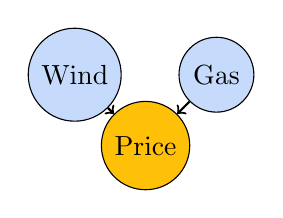
\begin{tikzpicture}[scale=0.6]
\node[draw, circle, fill=elecyellow] (price) at (0,0) {Price};
\node[draw, circle, fill=causalblue!30] (wind) at (-1.5,1.5) {Wind};
\node[draw, circle, fill=causalblue!30] (gas) at (1.5,1.5) {Gas};
\draw[->, thick] (wind) -- (price);
\draw[->, thick] (gas) -- (price);
\end{tikzpicture}
\end{center}
\begin{center}
\fcolorbox{reprogreen}{lightgray}{\parbox{0.9\textwidth}{\centering
\textbf{Benefit for Energy Trading:} Knowing that ``wind generation $\rightarrow$ price'' is causal (not just correlated) enables better hedging strategies and scenario analysis under different weather conditions.
}}
\end{center}
\end{frame}

%==============================================================================
\section{Data}

\begin{frame}{Data Description: European Electricity Markets}
\begin{columns}
\begin{column}{0.5\textwidth}
\textbf{Target Variables:}
\begin{itemize}
    \item \textbf{DE}: German day-ahead price (EUR/MWh)
    \item \textbf{FR}: French day-ahead price (EUR/MWh)
    \item \textbf{DE\_FR}: Price spread %(DE - FR, calculated)
\end{itemize}

\textbf{Explanatory Features (19 total):}
\begin{itemize}
    \item \textbf{Generation (9)}: Wind, Solar, Hydro, Nuclear, Gas, Coal, Lignite, Biomass (MW)
    \item \textbf{Load (1)}: Actual demand (MW)
    \item \textbf{Commodities (3)}: Natural Gas, Brent, WTI (prices)
    \item \textbf{Weather (6)}: Temperature, Wind, Radiation, Cloud, Precipitation
\end{itemize}
\end{column}

\begin{column}{0.5\textwidth}
\textbf{Data Statistics (Daily, 2015-2024):}
\begin{table}
\scriptsize
\begin{tabular}{l|ccc}
\toprule
& \textbf{DE} & \textbf{FR} & \textbf{Spread} \\
\midrule
Samples & 3,652 & 3,652 & 3,651 \\
Mean & 71 EUR & 78 EUR & -7 EUR \\
Std & 78 EUR & 88 EUR & 27 EUR \\
Min & -50 EUR & -9 EUR & -480 EUR \\
Max & 705 EUR & 740 EUR & 222 EUR \\
\bottomrule
\end{tabular}
\end{table}

\textbf{Key characteristics:}
\begin{itemize}
    \item Heavy tails (kurtosis: 13 DE, 12 FR, 42 spread)
    \item Strong autocorrelation (lag-1: 0.94, 0.97, 0.71)
    \item Prices right-skewed; spread left-skewed
\end{itemize}
\end{column}
\end{columns}
\end{frame}

%------------------------------------------------------------------------------
\begin{frame}{Power Generation Mix: Energy Transition (2015 $\rightarrow$ 2024)}
\begin{columns}
\begin{column}{0.5\textwidth}
\centering
\textbf{Germany (DE)}
\vspace{0.2cm}

\begin{columns}
\begin{column}{0.5\textwidth}
\centering
\small 2015
\includesvg[width=0.95\textwidth]{figures/generation_pie_de_2015}
\end{column}
\begin{column}{0.5\textwidth}
\centering
\small 2024
\includesvg[width=0.95\textwidth]{figures/generation_pie_de_2024}
\end{column}
\end{columns}
\end{column}

\begin{column}{0.5\textwidth}
\centering
\textbf{France (FR)}
\vspace{0.2cm}

\begin{columns}
\begin{column}{0.5\textwidth}
\centering
\small 2015
\includesvg[width=0.95\textwidth]{figures/generation_pie_fr_2015}
\end{column}
\begin{column}{0.5\textwidth}
\centering
\small 2024
\includesvg[width=0.95\textwidth]{figures/generation_pie_fr_2024}
\end{column}
\end{columns}
\end{column}
\end{columns}

\vspace{0.3cm}
\small
\textbf{Key changes:} DE: Nuclear phase-out (14\% $\rightarrow$ 0\%), wind doubles (21\% $\rightarrow$ 41\%). FR: Nuclear stable ($\sim$70\%).
\end{frame}

%------------------------------------------------------------------------------
\begin{frame}{Time Series: Germany Day-Ahead Prices (2015-2024)}
\begin{center}
\includesvg[height=0.85\textheight]{figures/de_price_weather_generation.svg}
\end{center}
\end{frame}

%------------------------------------------------------------------------------
\begin{frame}{Time Series: France Day-Ahead Prices (2015-2024)}
\begin{center}
\includesvg[height=0.85\textheight]{figures/fr_price_weather_generation.svg}
\end{center}
\end{frame}

%==============================================================================
\section{Literature Review}

\begin{frame}{Model Comparison: Capabilities}
\begin{table}
\centering
\small
\begin{adjustbox}{max width=\textwidth}
\begin{tabular}{l|cccccc}
\toprule
\textbf{Model} & \textbf{Regime} & \textbf{Causal} & \textbf{Temporal} & \textbf{Non-Linear} & \textbf{Interpretable} & \textbf{Scalable} \\
& \textbf{Switching} & \textbf{DAGs} & \textbf{Dynamics} & \textbf{Relations} & \textbf{Graphs} & \textbf{($>$50 feat.)} \\
\midrule
ARIMA/VAR & \textcolor{warnred}{\ding{55}} & \textcolor{warnred}{\ding{55}} & \textcolor{reprogreen}{\ding{51}} & \textcolor{warnred}{\ding{55}} & \textcolor{warnred}{\ding{55}} & \textcolor{reprogreen}{\ding{51}} \\
MS-VAR & \textcolor{reprogreen}{\ding{51}} & \textcolor{warnred}{\ding{55}} & \textcolor{reprogreen}{\ding{51}} & \textcolor{warnred}{\ding{55}} & \textcolor{warnred}{\ding{55}} & \textcolor{reprogreen}{\ding{51}} \\
NOTEARS/GOLEM & \textcolor{warnred}{\ding{55}} & \textcolor{reprogreen}{\ding{51}} & \textcolor{warnred}{\ding{55}} & \textcolor{reprogreen}{\ding{51}} & \textcolor{reprogreen}{\ding{51}} & \textcolor{reprogreen}{\ding{51}} \\
DYNOTEARS & \textcolor{warnred}{\ding{55}} & \textcolor{reprogreen}{\ding{51}} & \textcolor{reprogreen}{\ding{51}} & \textcolor{warnred}{\ding{55}} & \textcolor{reprogreen}{\ding{51}} & \textcolor{reprogreen}{\ding{51}} \\
DS3M & \textcolor{reprogreen}{\ding{51}} & \textcolor{warnred}{\ding{55}} & \textcolor{reprogreen}{\ding{51}} & \textcolor{reprogreen}{\ding{51}} & \textcolor{warnred}{\ding{55}} & \textcolor{reprogreen}{\ding{51}} \\
FANTOM & \textcolor{reprogreen}{\ding{51}} & \textcolor{reprogreen}{\ding{51}} & \textcolor{reprogreen}{\ding{51}} & \textcolor{reprogreen}{\ding{51}} & \textcolor{reprogreen}{\ding{51}} & \textcolor{warnred}{\ding{55}} \\
\midrule
\textbf{CaRS} & \textcolor{reprogreen}{\ding{51}} & \textcolor{reprogreen}{\ding{51}} & \textcolor{reprogreen}{\ding{51}} & \textcolor{reprogreen}{\ding{51}} & \textcolor{reprogreen}{\ding{51}} & \textcolor{reprogreen}{\ding{51}} \\
% \textbf{+ Shared Backbone} & \textcolor{reprogreen}{\ding{51}} & \textcolor{reprogreen}{\ding{51}} & \textcolor{reprogreen}{\ding{51}} & \textcolor{reprogreen}{\ding{51}} & \textcolor{reprogreen}{\ding{51}} & \textcolor{reprogreen}{\ding{51}} \\
\bottomrule
\end{tabular}
\end{adjustbox}
\end{table}

% {\scriptsize \textit{Scalability: FANTOM's normalizing flows cause OOM on 80GB GPUs with $>$50 features.}}

% \vspace{0.3cm}
\textbf{Key References:}
\begin{itemize}
    \item \textbf{DS3M} (Xu et al., 2021): Deep Switching State Space Model for time series
    \item \textbf{FANTOM} (Rahmani et al., 2025): Causal discovery with regime switching
    \item \textbf{NOTEARS} (Zheng et al., 2018): Differentiable DAG learning
\end{itemize}
\end{frame}

%==============================================================================
\section{Methodology}

%------------------------------------------------------------------------------
\begin{frame}{CaRS: Building Blocks \& Novelty}
\small
\begin{columns}
\begin{column}{0.48\textwidth}
\textcolor{paperblue}{\textbf{From DS3M (Temporal Backbone):}}
\begin{itemize}
    \item GRU encoder: $h_t = \text{GRU}(h_{t-1}, [X_t, Y_t])$
    \item Learnable Markov regime switching
    \item Continuous latent state $z_t$
\end{itemize}
\end{column}

\begin{column}{0.48\textwidth}
\textcolor{paperblue}{\textbf{From FANTOM (Causal Discovery):}}
\begin{itemize}
    \item ICGNN emission network
    \item Gumbel-Softmax DAG sampling
    \item NOTEARS acyclicity + sparsity constraints
\end{itemize}
\end{column}
\end{columns}

\vspace{0.4cm}
\begin{center}
\fcolorbox{reprogreen}{green!8}{\parbox{0.92\textwidth}{
\textbf{\textcolor{reprogreen}{CaRS Novelty --- Joint End-to-End Learning:}}\\[4pt]
The GRU hidden state $h_t$ simultaneously conditions:
\begin{enumerate}
    \item the \textbf{regime posterior} $P(d_t \mid h_t, d_{t-1})$ --- \textit{which} causal structure is active
    \item the \textbf{causal emission} $\hat{Y}_t = f_{\text{ICGNN}}(X_t, h_t, z_t, A^{(d_t)})$ --- \textit{how} to predict through the DAG
\end{enumerate}
\vspace{2pt}
Regimes, causal DAGs, and predictions are learned in a \textbf{single ELBO optimization} --- not a two-stage pipeline.
}}
\end{center}
\end{frame}

%------------------------------------------------------------------------------
\begin{frame}{Model Overview: CaRS}
\small
\begin{columns}
\begin{column}{0.5\textwidth}
\textbf{DS3M\_UV (Univariate)}
\begin{itemize}
    \item Only uses target $Y$
    \item Autoregressive regime switching
    \item Strong baseline for price forecasting
\end{itemize}

\vspace{0.3cm}
\textbf{DS3M\_MV (Multivariate)}
\begin{itemize}
    \item Uses features $X$ and target $Y$
    \item Black-box emission network
    \item No interpretable structure
\end{itemize}
\end{column}

\begin{column}{0.5\textwidth}
\textbf{CaRS (Ours)}
\begin{itemize}
    \item Combines SSM regime switching with causal discovery
    \item \textbf{Key innovation:} Enhances SSM with Invertible Contractive Graph Neural Network (ICGNN)%Replace DS3M's emission network with FANTOM's ICGNN
    \item Learns \textbf{sparse causal DAGs per regime}
\end{itemize}

% \vspace{0.1cm}
\textbf{FANTOM\_BEM (Baseline)}
\begin{itemize}
    \item Bayesian EM for regime detection
    \item Full FANTOM causal discovery
    \item Reference implementation
\end{itemize}
\end{column}
\end{columns}
\end{frame}

\begin{frame}{Model Overview: CaRS}
\begin{center}
\fcolorbox{causalblue}{lightgray}{\parbox{0.9\textwidth}{\centering
\textbf{Novelty:} CaRS jointly learns \textit{regime-switching causal DAGs} end-to-end within a deep state space---regimes and causal structure are discovered simultaneously, not in a two-stage pipeline. Each regime defines a Structural Equation Model (ICGNN + NOTEARS), so every prediction decomposes into \textit{interpretable directed causal edges} that change with market regime.
}}
\end{center}
\end{frame}

%------------------------------------------------------------------------------
\begin{frame}{Key Methodological Differences: DS3M vs FANTOM vs CaRS}
\begin{table}
\centering
\small
\begin{adjustbox}{max width=\textwidth}
\begin{tabular}{l|ccc}
\toprule
\textbf{Component} & \textbf{DS3M} & \textbf{FANTOM} & \textbf{CaRS (Ours)} \\
\midrule
\textbf{Temporal Encoding} & GRU & Lag-based (no recurrence) & GRU \\
\textbf{Regime Detection} & Markov (learnable) & Bayesian EM & Markov (learnable) \\
\textbf{State Space} & Continuous $z_t$ & \textcolor{warnred}{None} & Continuous $z_t$ \\
\textbf{Emission Model} & Black-box MLP & ICGNN & ICGNN \\
\textbf{Causal DAG Learning} & \textcolor{warnred}{None} & Gumbel-Softmax (per-regime) & Gumbel-Softmax (per-regime) \\
\textbf{Noise Modeling} & Gaussian & Cond. Norm. Flows & Gaussian$^*$ \\
\bottomrule
\end{tabular}    
\end{adjustbox}
\end{table}

{\scriptsize $^*$CaRS uses Gaussian noise for computational efficiency and numerical stability, enabling scalable training.} %Trade-off: less expressive than normalizing flows but more robust with larger feature sets.}

\vspace{0.1cm}
% \textbf{What each method contributes:}
% \vspace{0.1cm}
\begin{columns}
\begin{column}{0.33\textwidth}
\textcolor{paperblue}{\textbf{From DS3M:}}
\begin{itemize}
    \item GRU temporal encoding
    \item Learnable Markov regimes
    \item Continuous latent state
\end{itemize}
\end{column}

\begin{column}{0.33\textwidth}
\textcolor{paperblue}{\textbf{From FANTOM:}}
\begin{itemize}
    \item ICGNN architecture
    \item Differentiable DAG learning
    \item Sparsity constraints
\end{itemize}
\end{column}

\begin{column}{0.33\textwidth}
\textcolor{reprogreen}{\textbf{CaRS Innovation:}}
\begin{itemize}
    \item $h_t$ conditions regime posterior AND causal emission
    \item Joint end-to-end ELBO optimization
    \item Temporal + causal + interpretable
\end{itemize}
\end{column}
\end{columns}
\end{frame}

%------------------------------------------------------------------------------
\begin{frame}{The Joint Learning Mechanism}
\small
\begin{columns}
\begin{column}{0.52\textwidth}
\textcolor{reprogreen}{\textbf{CaRS: Joint End-to-End}}\\[4pt]
\begin{center}
\fcolorbox{reprogreen}{green!5}{\parbox{0.88\linewidth}{
\centering
$h_t = \text{GRU}(h_{t-1}, [X_t, Y_t])$\\[3pt]
{\scriptsize \textit{temporal context encodes full history}}\\[4pt]
$\swarrow \hspace{2.5cm} \searrow$\\[3pt]
$d_t \sim P(d \mid h_t, d_{t-1})$ \hfill $z_t \sim \mathcal{N}(\mu(h_t, d), \sigma(h_t, d))$\\[1pt]
{\scriptsize \textit{regime posterior}} \hfill {\scriptsize \textit{continuous latent}}\\[4pt]
$\searrow \hspace{2.5cm} \swarrow$\\[3pt]
$\hat{Y}_t = f_{\text{ICGNN}}(X_t, \mathbf{h_t}, z_t, A^{(d_t)})$\\[1pt]
{\scriptsize \textit{causal prediction through regime-specific DAG}}
}}
\end{center}
\vspace{2pt}
{\scriptsize $h_t$ informs \textbf{both} which regime is active \textbf{and} how to predict through the causal graph.}
\end{column}

\begin{column}{0.44\textwidth}
\textcolor{warnred}{\textbf{FANTOM: Two-Stage Pipeline}}\\[4pt]
\begin{center}
\fcolorbox{warnred}{red!5}{\parbox{0.88\linewidth}{
\centering
\textbf{Stage 1:}\\[1pt]
$\text{BEM}(Y_{1:T}) \rightarrow \{d_t\}$\\[1pt]
{\scriptsize \textit{regime labels from $Y$ alone}}\\[1pt]
{\scriptsize \textcolor{warnred}{No temporal state $h_t$}}\\[6pt]
\textbf{Stage 2:}\\[1pt]
$\text{FANTOM}(X, Y \mid d) \rightarrow A^{(d)}$\\[1pt]
{\scriptsize \textit{per-regime DAG, learned independently}}\\[1pt]
{\scriptsize \textcolor{warnred}{No cross-regime information flow}}
}}
\end{center}
\vspace{2pt}
{\scriptsize Regimes detected from $Y$ alone; DAGs learned independently per regime.}
\end{column}
\end{columns}

\vspace{0.2cm}
\begin{center}
\fcolorbox{reprogreen}{green!8}{\parbox{0.9\textwidth}{\centering
\scriptsize \textbf{Key difference:} In CaRS, temporal context ($h_t$) directly shapes causal structure --- the model discovers that causal relationships change \textit{because of} temporal dynamics, not just segments data into static regimes.
}}
\end{center}
\end{frame}

%==============================================================================
% NEW METHODOLOGY SLIDES: Problem Setup, SEM, Parameters, ELBO
%==============================================================================

\begin{frame}{Problem Setup: Modeling Electricity Prices}
\begin{columns}
\begin{column}{0.5\textwidth}
\textbf{Observed Variables:}
\begin{itemize}
    \item $X_t \in \mathbb{R}^{n}$: \textbf{Exogenous features} at time $t$
    \begin{itemize}
        \scriptsize
        \item Generation: Wind, Solar, Gas, Nuclear (MW)
        \item Commodities: Gas price, Brent, Carbon (EUR)
        \item Weather: Temperature, Wind speed, Radiation
    \end{itemize}
    \item $Y_t \in \mathbb{R}$: \textbf{Target variable} (electricity price, EUR/MWh)
\end{itemize}

\vspace{0.2cm}
\textbf{Data Structure:}
\begin{itemize}
    \item Time series: $(X_1, Y_1), (X_2, Y_2), \ldots, (X_T, Y_T)$
    \item Dimensions: $n = 19$ features, $T \approx 3{,}652$ days
\end{itemize}
\end{column}

\begin{column}{0.5\textwidth}
\textbf{Tasks:}
\begin{enumerate}
    \item \textbf{Estimation:} Given $X_{0:t}, Y_{0:t-1}$, estimate $Y_t$
    \item \textbf{Prediction:} Given $X_{0:t}, Y_{0:t}$, predict $Y_{t+1}$
    \item \textbf{Causal Discovery:} Which $X_t^{(i)} \rightarrow Y_t$?
\end{enumerate}

\vspace{0.3cm}
\begin{center}
\fcolorbox{warnred}{lightgray}{\parbox{0.9\linewidth}{\centering
\small \textbf{Key Challenge:}\\
Causal relationships \textit{change over time}!\\[2pt]
\scriptsize E.g., Wind's impact on price differs\\
in normal vs. crisis market conditions.
}}
\end{center}
\end{column}
\end{columns}
\end{frame}

%------------------------------------------------------------------------------
\begin{frame}{Structural Equation Model}
$Y_t$ is generated by a \textbf{regime-specific} structural equation:

\vspace{0.2cm}
\begin{center}
\fcolorbox{causalblue}{lightgray}{\parbox{0.85\textwidth}{\centering
\vspace{0.15cm}
$Y_t = f^{(d_t)}\left(\mathrm{Pa}_{G^{(d_t)}}(Y_t)\right) + g^{(d_t)}\left(\mathrm{Pa}_{G^{(d_t)}}(Y_t)\right) \cdot \epsilon_t$
\vspace{0.15cm}
}}
\end{center}

\vspace{0.2cm}
\textbf{Step-by-step breakdown:}
\begin{enumerate}
    \item $d_t \in \{1, \ldots, K\}$: Current \textbf{regime} %(e.g., normal market, crisis, high-renewable)
    \item $G^{(d_t)}$: The \textbf{causal DAG} active in regime $d_t$
    \item $\mathrm{Pa}_{G^{(d_t)}}(Y_t) \subseteq X_t$: \textbf{Causal parents} of $Y_t$ in the DAG
    \item $f^{(d_t)}(\cdot)$: \textbf{Mean function} (ICGNN) %--- predicts expected price
    \item $g^{(d_t)}(\cdot)$: \textbf{Variance function} --- captures heteroscedasticity
    \item $\epsilon_t \sim \mathcal{N}(0,1)$: Standardized noise
\end{enumerate}

\vspace{0.2cm}
\textbf{Example:} If Wind $\in \text{Pa}(Y_t)$ but Solar $\notin \text{Pa}(Y_t)$, then wind \textit{causally} affects price while solar does not (enforced via DAG mask $A^{(d_t)}$).
\end{frame}

%------------------------------------------------------------------------------
\begin{frame}{Model Parameters: What CaRS Learns}
\begin{columns}
\begin{column}{0.5\textwidth}
\textbf{Latent Variables (per timestep $t$):}
\begin{align*}
h_t &= \text{GRU}(h_{t-1}, [X_t, Y_t]) && \text{\scriptsize (hidden state)}\\
d_t &\in \{1, \ldots, K\} && \text{\scriptsize (discrete regime)}\\
z_t &\sim \mathcal{N}(\mu(h_t, d_t), \sigma(h_t, d_t)) && \text{\scriptsize (continuous latent)}
\end{align*}

\vspace{0.2cm}
\textbf{Structural Parameters (per regime $r$):}
\begin{align*}
A^{(r)} &\in [0,1]^{n \times n} && \text{\scriptsize (causal adjacency)}\\
\theta^{(r)} &= \{\psi^r, \vartheta^r\} && \text{\scriptsize (ICGNN weights)}
\end{align*}
\end{column}

\begin{column}{0.5\textwidth}
\textbf{Transition Parameters:}
\begin{align*}
\Phi &\in \mathbb{R}^{K \times K} && \text{\scriptsize (transition logits)}\\
P(d_t | d_{t-1}) &= \text{softmax}(\Phi)_{d_{t-1},:}
\end{align*}

\vspace{0.2cm}
\textbf{Emission (Final Prediction):}
\begin{equation*}
\hat{Y}_t = f_{\text{ICGNN}}(X_t, h_t, z_t, A^{(d_t)})
\end{equation*}

\vspace{0.3cm}
\begin{center}
\fcolorbox{reprogreen}{lightgray}{\parbox{0.9\linewidth}{\centering
\scriptsize \textbf{Learnable:} GRU weights, ICGNN $\theta^{(r)}$,\\
DAG params $\phi^{(r)}$, transitions $\Phi$
}}
\end{center}
\end{column}
\end{columns}
\end{frame}

%------------------------------------------------------------------------------
\begin{frame}{The Optimization Challenge: Why Direct MLE is Impossible}
\textbf{Goal:} Maximize the log-likelihood of observed data $(X, Y)_{1:T}$:
\begin{equation*}
\log p_\Theta(Y_{1:T} | X_{1:T}) = \log \int \sum_{d_{1:T}} p(Y, d, z, G \,|\, X) \, dz
\end{equation*}

\vspace{0.2cm}
\textbf{Problem: This integral is INTRACTABLE!}
\begin{columns}
\begin{column}{0.33\textwidth}
\textbf{1. Latent Regimes $d_t$}
\begin{itemize}
    \scriptsize
    \item $d_t$ is \textbf{unobserved}
    \item Must sum over $K^T$ sequences
    \item E.g., $3^{3652} \approx 10^{1742}$
\end{itemize}
\end{column}

\begin{column}{0.33\textwidth}
\textbf{2. Continuous Latents $z_t$}
\begin{itemize}
    \scriptsize
    \item Must integrate over all $z_t$ values
    \item Non-linear ICGNN: no closed form
\end{itemize}
\end{column}

\begin{column}{0.33\textwidth}
\textbf{3. Unknown DAGs $G^{(r)}$}
\begin{itemize}
    \scriptsize
    \item Structure is \textbf{also latent}
    \item $2^{n^2}$ possible graphs
    \item E.g., $2^{361} \approx 10^{109}$
\end{itemize}
\end{column}
\end{columns}

\vspace{0.3cm}
\begin{center}
\fcolorbox{causalblue}{lightgray}{\parbox{0.8\textwidth}{\centering
\textbf{Solution:} Instead of maximizing $\log p(Y|X)$ directly,\\
maximize a tractable \textbf{lower bound} (ELBO)
}}
\end{center}
\end{frame}

%------------------------------------------------------------------------------
\begin{frame}{Evidence Lower Bound (ELBO): Making Optimization Tractable}
\textbf{Key Identity} (Jensen's Inequality):
\begin{equation*}
\log p(Y|X) \geq \underbrace{\mathbb{E}_{q}[\log p(Y|X,z,d,G)]}_{\text{Reconstruction}} - \underbrace{\text{KL}[q(z,d,G) \,\|\, p(z,d,G)]}_{\text{Regularization}} = \text{ELBO}
\end{equation*}

\vspace{0.1cm}
\begin{columns}
\begin{column}{0.5\textwidth}
\textbf{The Variational Distribution $q$:}
\begin{itemize}
    \item $q(z_t | h_t, Y_t)$: \textbf{Gaussian} posterior for $z_t$
    \item $q(d_t | h_t, Y_t)$: \textbf{Categorical} posterior for regime
    \item $q_\phi(G^{(r)})$: \textbf{Factorized Bernoullis} for DAG edges
\end{itemize}

\vspace{0.1cm}
\textbf{What's special about $q$?}
\begin{itemize}
    \item Tractable: we can sample from it
    \item Learnable: parametrized by neural networks
    \item Approximates true posterior $p(\cdot | Y, X)$
\end{itemize}
\end{column}

\begin{column}{0.5\textwidth}
\textbf{Why ``Lower Bound''?}
\begin{itemize}
    \item ELBO $\leq \log p(Y|X)$ \textbf{always}
    \item Gap = $\text{KL}[q \,\|\, p(\cdot|Y,X)] \geq 0$
\end{itemize}

\vspace{0.1cm}
\textbf{When is the bound tight?}
\begin{itemize}
    \item When $q = p(z,d,G \,|\, Y,X)$ exactly
    \item In practice: optimize $q$ to minimize gap
\end{itemize}

% \vspace{0.2cm}
\begin{center}
\fcolorbox{reprogreen}{lightgray}{\parbox{0.9\linewidth}{\centering
\scriptsize \textbf{Training:} Maximize ELBO w.r.t.\\
model params $\Theta$ \textit{and} variational params $\phi$
}}
\end{center}
\end{column}
\end{columns}
\end{frame}

%------------------------------------------------------------------------------
\begin{frame}{Sampling and Reparametrization Tricks}
\textbf{CaRS ELBO (expanded):}
\begin{equation*}
\mathcal{L} = \underbrace{\mathbb{E}_{q}[\log p(Y|X,z,d,A)]}_{\text{Reconstruction}} - \underbrace{\text{KL}[q(z) \| p(z)]}_{\text{Continuous}} - \underbrace{\text{KL}[q(d) \| p(d|d_{t-1})]}_{\text{Discrete}} + \underbrace{\lambda_{\text{dag}} h(A) + \lambda_{\text{sp}} \|A\|_1}_{\text{DAG Constraints}}
\end{equation*}

\begin{columns}
\begin{column}{0.5\textwidth}
\textbf{Reparametrization Trick} (continuous $z_t$):
\begin{enumerate}
    \item Sample $\epsilon \sim \mathcal{N}(0, I)$
    \item Compute $z_t = \mu(h_t, d_t) + \sigma(h_t, d_t) \odot \epsilon$
    \item \textcolor{reprogreen}{Gradients flow through $\mu, \sigma$!}
\end{enumerate}

% \vspace{0.1cm}
\textbf{Gumbel-Softmax} (discrete DAG $A$):
\begin{itemize}
    \item DAG edges are Bernoulli: $A_{ij} \in \{0, 1\}$
    \item Relaxation: $\text{softmax}\!\left(\frac{\log \pi + G}{\tau}\right)$
    \item $G \sim \text{Gumbel}(0,1)$; $\tau$ = temperature
\end{itemize}
\end{column}

\begin{column}{0.5\textwidth}
\textbf{Monte Carlo Estimation:}
\begin{equation*}
\mathbb{E}_q[f(z)] \approx \frac{1}{N}\sum_{i=1}^N f(z^{(i)}), \quad z^{(i)} \sim q
\end{equation*}
\begin{itemize}
    \item Training: $N=1$ sample (unbiased gradient)
    \item Inference: $N > 1$ for uncertainty
\end{itemize}

% \vspace{0.1cm}
\textbf{DAG Acyclicity} (NOTEARS):
\begin{equation*}
h(A) = \text{tr}(e^{A \odot A}) - n = 0
\end{equation*}
\scriptsize Ensures no directed cycles in learned graph.
\end{column}
\end{columns}
\end{frame}

\begin{frame}{Sampling and Reparametrization Tricks}
% \vspace{0.1cm}
\scriptsize DAG Acyclicity: Ensures no directed cycles in learned graph.
{\scriptsize See Appendix for detailed derivations of KL terms, Gumbel-Softmax, and NOTEARS constraint.}
\end{frame}

%------------------------------------------------------------------------------
\begin{frame}{CaRS: Architecture}
\begin{center}
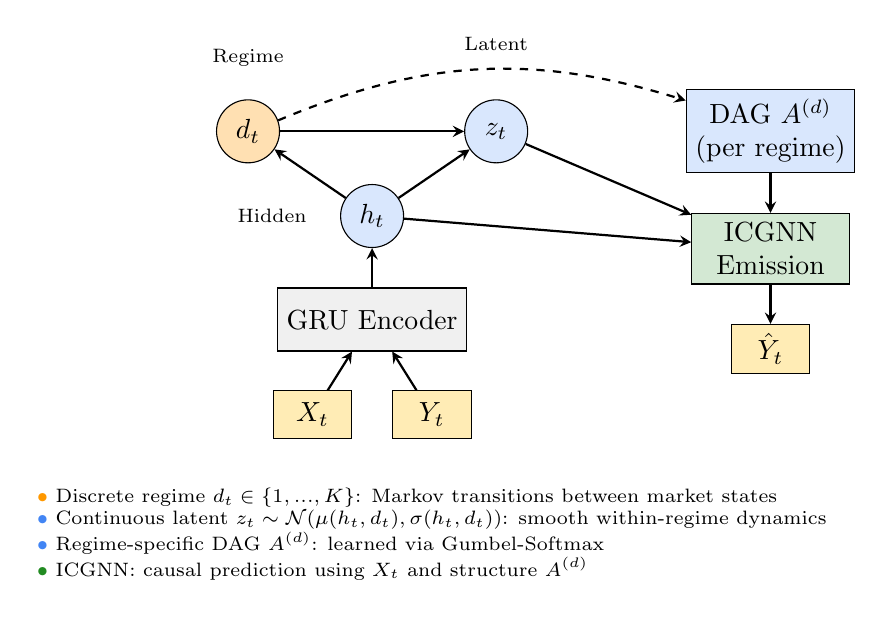
\begin{tikzpicture}[
    node distance=1.2cm,
    block/.style={draw, rectangle, minimum width=2cm, minimum height=0.8cm, align=center},
    latent/.style={draw, circle, minimum size=0.8cm, fill=causalblue!20},
    observed/.style={draw, rectangle, minimum width=1cm, minimum height=0.6cm, fill=elecyellow!30},
    arrow/.style={->, thick, >=stealth}
]

% Input
\node[observed] (x) {$X_t$};
\node[observed, right=0.5cm of x] (y) {$Y_t$};

% GRU Encoder
\node[block, above=0.8cm of $(x)!0.5!(y)$, fill=lightgray] (gru) {GRU Encoder};
\draw[arrow] (x) -- (gru);
\draw[arrow] (y) -- (gru);

% Hidden state
\node[latent, above=0.5cm of gru] (h) {$h_t$};
\node[left=0.3cm of h, font=\scriptsize] {Hidden};
\draw[arrow] (gru) -- (h);

% Discrete regime
\node[latent, above left=0.5cm and 1cm of h, fill=regimeorange!30] (d) {$d_t$};
\node[above=0.3cm of d, font=\scriptsize] {Regime};
\draw[arrow] (h) -- (d);

% Continuous latent
\node[latent, above right=0.5cm and 1cm of h] (z) {$z_t$};
\node[above=0.5cm of z, font=\scriptsize] {Latent};
\draw[arrow] (h) -- (z);
\draw[arrow] (d) -- (z);

% DAG per regime
\node[block, right=2cm of z, fill=causalblue!20] (dag) {DAG $A^{(d)}$\\(per regime)};
\draw[arrow, dashed] (d) to[bend left=20] (dag);

% ICGNN
\node[block, below=0.5cm of dag, fill=reprogreen!20] (icgnn) {ICGNN\\Emission};
\draw[arrow] (dag) -- (icgnn);
\draw[arrow] (z) -- (icgnn);
\draw[arrow] (h) -- (icgnn);

% Output
\node[observed, below=0.5cm of icgnn] (yhat) {$\hat{Y}_t$};
\draw[arrow] (icgnn) -- (yhat);

% Input to ICGNN
% \node[left=1cm of icgnn] (xin) {};
% \draw[arrow] (x.east) -| ($(icgnn.west)-(0.3,0)$) -- (icgnn.west);

% Legend
\node[below=0.5cm of y, font=\scriptsize, align=left] {
    \textcolor{regimeorange}{$\bullet$} Discrete regime $d_t \in \{1,...,K\}$: Markov transitions between market states\\
    \textcolor{causalblue}{$\bullet$} Continuous latent $z_t \sim \mathcal{N}(\mu(h_t,d_t), \sigma(h_t,d_t))$: smooth within-regime dynamics\\
    \textcolor{causalblue}{$\bullet$} Regime-specific DAG $A^{(d)}$: learned via Gumbel-Softmax\\
    \textcolor{reprogreen}{$\bullet$} ICGNN: causal prediction using $X_t$ and structure $A^{(d)}$
};

\end{tikzpicture}
\end{center}
\end{frame}

%------------------------------------------------------------------------------
\begin{frame}{CaRS: Detailed Architecture with Shared Backbone}
\begin{center}
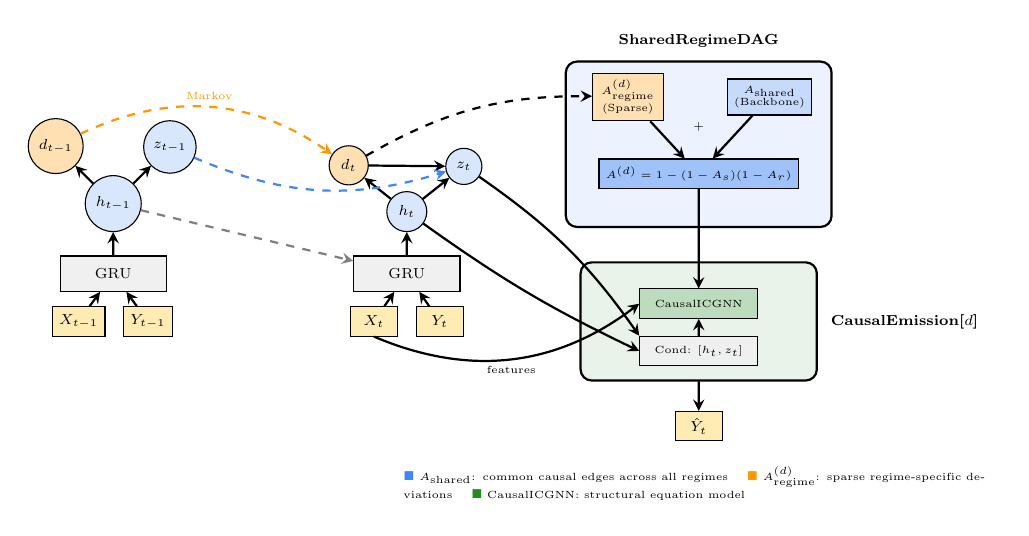
\begin{tikzpicture}[
    scale=0.75, transform shape,
    node distance=0.8cm,
    block/.style={draw, rectangle, minimum width=1.8cm, minimum height=0.6cm, align=center, font=\scriptsize},
    smallblock/.style={draw, rectangle, minimum width=1.2cm, minimum height=0.5cm, align=center, font=\tiny},
    latent/.style={draw, circle, minimum size=0.6cm, fill=causalblue!20, font=\scriptsize},
    observed/.style={draw, rectangle, minimum width=0.8cm, minimum height=0.5cm, fill=elecyellow!30, font=\scriptsize},
    bigbox/.style={draw, rectangle, rounded corners, thick},
    arrow/.style={->, thick, >=stealth},
    dashedarrow/.style={->, dashed, thick, >=stealth}
]

% Time t-1 column (left)
\node[observed] (xprev) at (-5, 0) {$X_{t-1}$};
\node[observed, right=0.3cm of xprev] (yprev) {$Y_{t-1}$};
\node[block, above=0.5cm of $(xprev)!0.5!(yprev)$, fill=lightgray] (gruprev) {GRU};
\node[latent, above=0.4cm of gruprev] (hprev) {$h_{t-1}$};
\node[latent, above left=0.3cm and 0.3cm of hprev, fill=regimeorange!30, minimum size=0.5cm] (dprev) {$d_{t-1}$};
\node[latent, above right=0.3cm and 0.3cm of hprev, minimum size=0.5cm] (zprev) {$z_{t-1}$};

\draw[arrow] (xprev) -- (gruprev);
\draw[arrow] (yprev) -- (gruprev);
\draw[arrow] (gruprev) -- (hprev);
\draw[arrow] (hprev) -- (dprev);
\draw[arrow] (hprev) -- (zprev);

% Time t column (center)
\node[observed] (x) at (0, 0) {$X_t$};
\node[observed, right=0.3cm of x] (y) {$Y_t$};
\node[block, above=0.5cm of $(x)!0.5!(y)$, fill=lightgray] (gru) {GRU};
\node[latent, above=0.4cm of gru] (h) {$h_t$};
\node[latent, above left=0.3cm and 0.5cm of h, fill=regimeorange!30] (d) {$d_t$};
\node[latent, above right=0.3cm and 0.5cm of h] (z) {$z_t$};

\draw[arrow] (x) -- (gru);
\draw[arrow] (y) -- (gru);
\draw[arrow] (gru) -- (h);
\draw[arrow] (h) -- (d);
\draw[arrow] (h) -- (z);
\draw[arrow] (d) -- (z);

% Temporal connections
\draw[dashedarrow, gray] (hprev) -- (gru);
\draw[dashedarrow, regimeorange] (dprev) to[bend left=30] node[above, font=\tiny] {Markov} (d);
\draw[dashedarrow, causalblue] (zprev) to[bend right=20] (z);

% SharedRegimeDAG box (right side)
\node[bigbox, fill=causalblue!10, minimum width=4.5cm, minimum height=2.8cm] (dagbox) at (5.5, 3) {};
\node[above=0.1cm of dagbox.north, font=\scriptsize\bfseries] {SharedRegimeDAG};

% Inside DAG box
\node[smallblock, fill=causalblue!30] (ashared) at (6.7, 3.8) {$A_{\text{shared}}$\\(Backbone)};
\node[smallblock, fill=regimeorange!30] (aregime) at (4.3, 3.8) {$A_{\text{regime}}^{(d)}$\\(Sparse)};
\node[font=\tiny] at (5.5, 3.3) {$+$};
\node[smallblock, fill=causalblue!50, minimum width=2.5cm] (acombined) at (5.5, 2.5) {$A^{(d)} = 1-(1-A_s)(1-A_r)$};

\draw[arrow] (ashared) -- (acombined);
\draw[arrow] (aregime) -- (acombined);
\draw[dashedarrow] (d) to[bend left=15] (aregime);

% CausalEmission box
\node[bigbox, fill=reprogreen!10, minimum width=4cm, minimum height=2cm] (emissionbox) at (5.5, 0) {};
\node[right=0.1cm of emissionbox.east, font=\scriptsize\bfseries] {CausalEmission[$d$]};

% Inside Emission box
\node[smallblock, fill=reprogreen!30, minimum width=2cm] (icgnn) at (5.5, 0.3) {CausalICGNN};
\node[smallblock, fill=lightgray, minimum width=2cm] (condnet) at (5.5, -0.5) {Cond: $[h_t, z_t]$};

\draw[arrow] (acombined) -- (icgnn);
\draw[arrow] (h) to[bend right=5] (condnet.west);
\draw[arrow] (z) to[bend left=10] (condnet.north west);
\draw[arrow] (condnet) -- (icgnn);

% X input to ICGNN
\draw[arrow] (x.south) to[bend right=30] node[below, font=\tiny] {features} (icgnn.west);

% Output
\node[observed, below=0.5cm of emissionbox] (yhat) {$\hat{Y}_t$};
\draw[arrow] (emissionbox) -- (yhat);

% Legend
\node[below=0.3cm of yhat, font=\tiny, align=left, text width=10cm] {
    \textcolor{causalblue}{$\blacksquare$} $A_{\text{shared}}$: common causal edges across all regimes \quad
    \textcolor{regimeorange}{$\blacksquare$} $A_{\text{regime}}^{(d)}$: sparse regime-specific deviations \quad
    \textcolor{reprogreen}{$\blacksquare$} CausalICGNN: structural equation model
};

\end{tikzpicture}
\end{center}
\end{frame}

%------------------------------------------------------------------------------
\begin{frame}{CausalICGNN: Internal Architecture}
\begin{center}
\begin{adjustbox}{height=0.85\textheight}
\begin{tikzpicture}[
    scale=0.8, transform shape,
    node distance=0.6cm,
    datablock/.style={draw, rectangle, minimum width=3cm, minimum height=0.6cm, align=center, font=\scriptsize, fill=elecyellow!20},
    netblock/.style={draw, rectangle, rounded corners, minimum width=3.5cm, minimum height=0.8cm, align=center, font=\scriptsize, fill=causalblue!20},
    opblock/.style={draw, rectangle, minimum width=3cm, minimum height=0.6cm, align=center, font=\scriptsize, fill=reprogreen!20},
    layerblock/.style={draw, rectangle, minimum width=2.5cm, minimum height=0.4cm, align=center, font=\tiny, fill=lightgray},
    arrow/.style={->, thick, >=stealth},
    annot/.style={font=\tiny, text=gray}
]

% Input
\node[datablock] (input) at (0, 6) {Input: $X \in \mathbb{R}^{B \times (L+1) \times n}$};
\node[annot, right=0.3cm of input] {$B$: batch, $L$: lag, $n$: nodes};

% Node Embeddings
\node[netblock, below=0.6cm of input, fill=regimeorange!20] (embed) {Node Embeddings $E$};
\node[annot, right=0.3cm of embed] {$E \in \mathbb{R}^{(L+1) \times n \times d}$ (learnable)};

% Concatenation
\node[opblock, below=0.6cm of embed] (concat) {Concatenate $[X_{\text{exp}}, E]$};
\node[annot, right=0.3cm of concat] {Shape: $[B, L{+}1, n, n, d{+}n]$};

% Encoder g
\node[netblock, below=0.6cm of concat, minimum height=1.4cm] (encoder) {
    \begin{tabular}{c}
    \textbf{Encoder Network} $g$ \\[2pt]
    \begin{tikzpicture}[scale=0.6]
        \node[layerblock] (l1) at (0,0) {FC $\to$ LN $\to$ LeakyReLU};
        \node[layerblock, below=0.15cm of l1] (l2) {FC $\to$ LN $\to$ LeakyReLU};
        \node[layerblock, below=0.15cm of l2] (l3) {FC $\to$ Output$(d)$};
    \end{tikzpicture}
    \end{tabular}
};
\node[annot, right=0.3cm of encoder] {$h = g(X, E) \in \mathbb{R}^{B \times (L{+}1) \times n \times n \times d}$};

% Message Aggregation
\node[opblock, below=0.8cm of encoder, minimum height=1.2cm, minimum width=4cm, fill=causalblue!30] (agg) {
    \begin{tabular}{c}
    \textbf{Weighted Message Aggregation} \\[2pt]
    $h_{\text{agg}} = \sum_j (W \odot A)_{ij} \cdot h_j$
    \end{tabular}
};
\node[annot, right=0.3cm of agg, align=left] {$W$: learned weights\\$A$: DAG (Gumbel)};

% Side inputs to aggregation
\node[datablock, left=1.5cm of agg, minimum width=1.5cm, fill=causalblue!40] (W) {$W$};
\node[datablock, left=1.5cm of W, minimum width=1.5cm, fill=regimeorange!40] (A) {$A^{(d)}$};
\draw[arrow] (W) -- (agg);
\draw[arrow] (A) -- (W);

% Decoder f
\node[netblock, below=0.8cm of agg, minimum height=1.4cm] (decoder) {
    \begin{tabular}{c}
    \textbf{Decoder Network} $f$ \\[2pt]
    \begin{tikzpicture}[scale=0.6]
        \node[layerblock] (l1) at (0,0) {FC $\to$ LN $\to$ LeakyReLU};
        \node[layerblock, below=0.15cm of l1] (l2) {FC $\to$ LN $\to$ LeakyReLU};
        \node[layerblock, below=0.15cm of l2] (l3) {FC $\to$ Output$(n)$};
    \end{tikzpicture}
    \end{tabular}
};
\node[annot, right=0.3cm of decoder] {$\hat{y} = f(E, h_{\text{agg}}) \in \mathbb{R}^{B \times n}$};

% Output
\node[datablock, below=0.8cm of decoder, fill=reprogreen!30] (output) {Predictions: $\hat{y} \in \mathbb{R}^{B \times n}$};

% Variance branch (optional)
\node[netblock, right=3cm of decoder, minimum width=2cm, minimum height=0.8cm, fill=gray!20, font=\tiny] (var) {Variance\\$g_{\text{var}}, f_{\text{var}}$};
\node[datablock, below=0.4cm of var, minimum width=1.5cm, fill=gray!30, font=\tiny] (varout) {$\sigma^2$};
\draw[arrow, gray] (agg.south east) to[bend left=20] (var.north);
\draw[arrow, gray] (var) -- (varout);
\node[annot, right=0.2cm of var] {(heteroscedastic)};

% Arrows
\draw[arrow] (input) -- (embed);
\draw[arrow] (embed) -- (concat);
\draw[arrow] (concat) -- (encoder);
\draw[arrow] (encoder) -- (agg);
\draw[arrow] (agg) -- (decoder);
\draw[arrow] (decoder) -- (output);

% Skip connection from embed to decoder
\draw[arrow, dashed, gray] (embed.west) to[out=180, in=180] node[left, font=\tiny] {$E$} (decoder.west);

\end{tikzpicture}
\end{adjustbox}
\end{center}
\end{frame}

%------------------------------------------------------------------------------
% NOTE: ELBO slide content moved to new methodology section (before Architecture)
%------------------------------------------------------------------------------
\begin{frame}{Understanding Latent Variables in CaRS}
\begin{columns}
\begin{column}{0.5\textwidth}
\textbf{Hidden State $h_t$} (GRU output)
\begin{itemize}
    \item Encodes \textbf{temporal memory} from past observations
    \item $h_t = \text{GRU}(h_{t-1}, [X_t, Y_t])$
    \item Captures autocorrelation and trends
    \item Deterministic given input sequence
\end{itemize}

\vspace{0.3cm}
\textbf{Discrete Regime $d_t$} (Markov)
\begin{itemize}
    \item Indicates \textbf{which market regime} is active
    \item $d_t \in \{1, 2, ..., K\}$
    \item Transitions: $P(d_t | d_{t-1}) = \text{softmax}(\Phi)$
    \item Selects which causal DAG $A^{(d)}$ to use
\end{itemize}
\end{column}

\begin{column}{0.5\textwidth}
\textbf{Continuous Latent $z_t$} (Gaussian)
\begin{itemize}
    \item Captures \textbf{smooth within-regime variation}
    \item $z_t \sim \mathcal{N}(\mu(h_t, d_t), \sigma(h_t, d_t))$
    \item Enables \textbf{Monte Carlo uncertainty quantification}
    \item At inference: sample $n$ times $\rightarrow$ mean $\pm$ std
\end{itemize}

\vspace{0.3cm}
\textbf{How They Interact:}
\begin{enumerate}
    \item $h_t$ summarizes temporal context
    \item $d_t$ determines regime (DAG selection)
    \item $z_t$ adds within-regime variability
    \item ICGNN combines all to predict $\hat{Y}_t$
\end{enumerate}
\end{column}
\end{columns}
\end{frame}

\begin{frame}{Target Output $\hat{Y}_t$ in CaRS}
\vspace{0.3cm}
\begin{center}
\fcolorbox{causalblue}{lightgray}{\parbox{0.85\textwidth}{\centering
$\hat{Y}_t = f_{\text{ICGNN}}(X_t, h_t, z_t, A^{(d_t)})$ where $A^{(d_t)}$ is the regime-specific causal graph
}}
\end{center}

\vspace{0.3cm}
\textbf{Uncertainty Quantification:}
\begin{itemize}
    \item CaRS provides \textbf{explicit predictive uncertainty} via Gaussian output
    \item Training: $p(Y_t | \cdot) = \mathcal{N}(\mu_t, \sigma_t)$ with learned heteroscedastic variance
    \item Inference: Monte Carlo sampling over $z_t$ yields prediction intervals
    \item Output: $(\hat{Y}_t, \hat{\sigma}_t)$ --- point estimate with uncertainty
\end{itemize}
\end{frame}

%==============================================================================
\section{Numerical Results}

\begin{frame}{Results: Estimation Task (Spearman $\rho$)}
\begin{table}
\centering
\small
\begin{adjustbox}{max width=\textwidth}
\begin{tabular}{l|cc|cc|cc}
\toprule
& \multicolumn{2}{c|}{\textbf{DE}} & \multicolumn{2}{c|}{\textbf{FR}} & \multicolumn{2}{c}{\textbf{DE\_FR}} \\
\textbf{Model} & d=2 & d=3 & d=2 & d=3 & d=2 & d=3 \\
\midrule
DS3M\_UV & \textbf{.78}$_{\pm.38}$ & .58$_{\pm.43}$ & .69$_{\pm.40}$ & \textbf{.93}$_{\pm.02}$ & .45$_{\pm.32}$ & .25$_{\pm.34}$ \\
DS3M\_MV & .41$_{\pm.46}$ & .58$_{\pm.49}$ & .75$_{\pm.37}$ & .44$_{\pm.42}$ & .34$_{\pm.40}$ & .24$_{\pm.27}$ \\
FANTOM\_BEM & .61$_{\pm.20}$ & \textbf{.92}$_{\pm.05}$ & \textbf{.83}$_{\pm.18}$ & .89$_{\pm.08}$ & \textbf{.55}$_{\pm.39}$ & \textbf{.69}$_{\pm.14}$ \\
\midrule
\textbf{CaRS} & .74$_{\pm.06}$ & .72$_{\pm.06}$ & .43$_{\pm.12}$ & .47$_{\pm.08}$ & .44$_{\pm.11}$ & .47$_{\pm.19}$ \\
\bottomrule
\end{tabular}
\end{adjustbox}
\end{table}

% {\scriptsize \textit{d=4 excluded due to regime collapse ($>$95\% of runs collapse to 1-2 regimes).}}

\vspace{0.2cm}
\textbf{Key Findings:}
\begin{itemize}
    \item \textbf{DE:} FANTOM\_BEM achieves $\rho = 0.92$ (d=3), highest among all models
    \item \textbf{FR:} DS3M\_UV strong ($\rho = 0.93$) for d=3; FANTOM\_BEM best for d=2 ($.83$)
    \item \textbf{DE\_FR:} FANTOM\_BEM best ($\rho = 0.55$--$0.69$)
    \item \textbf{CaRS:} Most stable across seeds ($\sigma = 0.06$--$0.19$ vs DS3M $\sigma = 0.27$--$0.49$)
\end{itemize}
\end{frame}

%------------------------------------------------------------------------------
\begin{frame}{Results: Estimation Task (RMSE)}
\begin{table}
\centering
\small
\begin{adjustbox}{max width=\textwidth}
\begin{tabular}{l|cc|cc|cc}
\toprule
& \multicolumn{2}{c|}{\textbf{DE}} & \multicolumn{2}{c|}{\textbf{FR}} & \multicolumn{2}{c}{\textbf{DE\_FR}} \\
\textbf{Model} & d=2 & d=3 & d=2 & d=3 & d=2 & d=3 \\
\midrule
DS3M\_UV & \textbf{190}$_{\pm10}$ & \textbf{199}$_{\pm11}$ & 103$_{\pm15}$ & \textbf{96}$_{\pm10}$ & \textbf{1375}$_{\pm20}$ & \textbf{1412}$_{\pm69}$ \\
DS3M\_MV & 199$_{\pm14}$ & 201$_{\pm6}$ & \textbf{103}$_{\pm12}$ & 108$_{\pm14}$ & 1395$_{\pm32}$ & 1386$_{\pm31}$ \\
FANTOM\_BEM & 12883$_{\pm10852}$ & 21580$_{\pm11157}$ & 4508$_{\pm1971}$ & 4110$_{\pm1953}$ & 46187$_{\pm21589}$ & 81941$_{\pm111418}$ \\
\midrule
\textbf{CaRS} & 205$_{\pm1}$ & 205$_{\pm1}$ & 117$_{\pm2}$ & 116$_{\pm1}$ & 1370$_{\pm3}$ & 1376$_{\pm6}$ \\
\bottomrule
\end{tabular}
\end{adjustbox}
\end{table}

\vspace{0.2cm}
{\scriptsize \textit{RMSE in EUR/MWh for DE/FR, spread units for DE\_FR.}} %d=4 excluded (regime collapse).}}

\vspace{0.2cm}
\textbf{Key Findings:}
\begin{itemize}
    \item \textbf{DS3M models}: Comparable RMSE ($\sim$190-206 for DE, $\sim$100-117 for FR)
    \item \textbf{FANTOM\_BEM}: Very high RMSE due to different prediction scale (raw price vs returns)
    \item \textbf{CaRS}: Most stable RMSE with very low variance ($\pm$1-14)
\end{itemize}
\end{frame}

%------------------------------------------------------------------------------
\begin{frame}{Results: Estimation Task (Directional Accuracy)}
\begin{table}
\centering
\small
\begin{adjustbox}{max width=\textwidth}
\begin{tabular}{l|cc|cc|cc}
\toprule
& \multicolumn{2}{c|}{\textbf{DE}} & \multicolumn{2}{c|}{\textbf{FR}} & \multicolumn{2}{c}{\textbf{DE\_FR}} \\
\textbf{Model} & d=2 & d=3 & d=2 & d=3 & d=2 & d=3 \\
\midrule
DS3M\_UV & \textbf{.84}$_{\pm.19}$ & .72$_{\pm.23}$ & .75$_{\pm.23}$ & \textbf{.90}$_{\pm.02}$ & .65$_{\pm.11}$ & .64$_{\pm.11}$ \\
DS3M\_MV & .68$_{\pm.16}$ & \textbf{.75}$_{\pm.24}$ & \textbf{.80}$_{\pm.15}$ & .68$_{\pm.21}$ & .56$_{\pm.07}$ & .59$_{\pm.11}$ \\
FANTOM\_BEM & .51$_{\pm.04}$ & .52$_{\pm.03}$ & .51$_{\pm.04}$ & .49$_{\pm.04}$ & .50$_{\pm.01}$ & .52$_{\pm.07}$ \\
\midrule
\textbf{CaRS} & .73$_{\pm.05}$ & .66$_{\pm.11}$ & .63$_{\pm.06}$ & .61$_{\pm.08}$ & \textbf{.64}$_{\pm.05}$ & \textbf{.67}$_{\pm.08}$ \\
\bottomrule
\end{tabular}
\end{adjustbox}
\end{table}

\vspace{0.2cm}
{\scriptsize \textit{Directional accuracy = fraction of correct price movement direction predictions.}} %d=4 excluded.}}

\vspace{0.2cm}
\textbf{Key Findings:}
\begin{itemize}
    \item \textbf{FR d=3:} DS3M\_UV achieves 90\% directional accuracy -- strong autoregressive signal
    \item \textbf{FANTOM\_BEM}: Near-random (50\%) directional accuracy despite reasonable Spearman
    \item \textbf{CaRS}: Consistent 61--73\% accuracy ($\sigma = 0.05$--$0.11$ vs DS3M $\sigma = 0.15$--$0.24$)
\end{itemize}
\end{frame}

%==============================================================================
\begin{frame}{Results: Prediction Task (Spearman $\rho$)}
\begin{table}
\centering
\small
\begin{adjustbox}{max width=\textwidth}
\begin{tabular}{l|cc|cc|cc}
\toprule
& \multicolumn{2}{c|}{\textbf{DE}} & \multicolumn{2}{c|}{\textbf{FR}} & \multicolumn{2}{c}{\textbf{DE\_FR}} \\
\textbf{Model} & d=2 & d=3 & d=2 & d=3 & d=2 & d=3 \\
\midrule
DS3M\_UV & .27$_{\pm.12}$ & .13$_{\pm.22}$ & .25$_{\pm.17}$ & .08$_{\pm.15}$ & .11$_{\pm.07}$ & .11$_{\pm.10}$ \\
DS3M\_MV & .29$_{\pm.26}$ & .27$_{\pm.23}$ & .33$_{\pm.25}$ & .25$_{\pm.24}$ & .11$_{\pm.11}$ & .07$_{\pm.08}$ \\
FANTOM\_BEM & \textbf{.82}$_{\pm.18}$ & \textbf{.93}$_{\pm.03}$ & \textbf{.81}$_{\pm.18}$ & \textbf{.93}$_{\pm.02}$ & \textbf{.64}$_{\pm.09}$ & \textbf{.69}$_{\pm.11}$ \\
\midrule
\textbf{CaRS} & .45$_{\pm.05}$ & .44$_{\pm.09}$ & .42$_{\pm.07}$ & .44$_{\pm.02}$ & .17$_{\pm.05}$ & .17$_{\pm.05}$ \\
\bottomrule
\end{tabular}
\end{adjustbox}
\end{table}

% {\scriptsize \textit{Results aggregated over 5 seeds.}} %d=4 excluded (regime collapse).}}

\vspace{0.2cm}
\textbf{Key Findings:}
\begin{itemize}
    \item \textbf{FANTOM\_BEM dominates:} Very high $\rho$ (0.81--0.93) across all configurations
    \item \textbf{But:} High Spearman with $\sim$50\% directional accuracy suggests overfitting to trends
    \item \textbf{CaRS:} Moderate Spearman (0.17--0.45) but better directional accuracy (55--65\%)
\end{itemize}
\end{frame}

%------------------------------------------------------------------------------
\begin{frame}{Results: Prediction Task (RMSE)}
\begin{table}
\centering
\small
\begin{adjustbox}{max width=\textwidth}
\begin{tabular}{l|cc|cc|cc}
\toprule
& \multicolumn{2}{c|}{\textbf{DE}} & \multicolumn{2}{c|}{\textbf{FR}} & \multicolumn{2}{c}{\textbf{DE\_FR}} \\
\textbf{Model} & d=2 & d=3 & d=2 & d=3 & d=2 & d=3 \\
\midrule
DS3M\_UV & \textbf{196}$_{\pm7}$ & 205$_{\pm5}$ & \textbf{112}$_{\pm5}$ & \textbf{115}$_{\pm6}$ & 1419$_{\pm24}$ & 1419$_{\pm11}$ \\
DS3M\_MV & 202$_{\pm7}$ & \textbf{204}$_{\pm3}$ & 114$_{\pm4}$ & 114$_{\pm5}$ & 1416$_{\pm11}$ & 1419$_{\pm25}$ \\
FANTOM\_BEM & 6837$_{\pm7818}$ & 25130$_{\pm14301}$ & 4630$_{\pm1439}$ & 2963$_{\pm1077}$ & 72240$_{\pm85922}$ & 51741$_{\pm26566}$ \\
\midrule
\textbf{CaRS} & 205$_{\pm1}$ & 206$_{\pm1}$ & 116$_{\pm1}$ & 116$_{\pm0}$ & \textbf{1392}$_{\pm3}$ & \textbf{1394}$_{\pm4}$ \\
\bottomrule
\end{tabular}
\end{adjustbox}
\end{table}

\vspace{0.2cm}
{\scriptsize \textit{RMSE in EUR/MWh for DE/FR, spread units for DE\_FR.}} %d=4 excluded.}}

\vspace{0.2cm}
\textbf{Key Findings:}
\begin{itemize}
    \item \textbf{DS3M models}: Similar RMSE ($\sim$196-206 for DE, $\sim$112-116 for FR)
    \item \textbf{CaRS}: Most stable RMSE with very low variance ($\pm$1-4)
    \item \textbf{FANTOM\_BEM}: High RMSE variance indicates unstable predictions
\end{itemize}
\end{frame}

%------------------------------------------------------------------------------
\begin{frame}{Results: Prediction Task (Directional Accuracy)}
\begin{table}
\centering
\small
\begin{adjustbox}{max width=\textwidth}
\begin{tabular}{l|cc|cc|cc}
\toprule
& \multicolumn{2}{c|}{\textbf{DE}} & \multicolumn{2}{c|}{\textbf{FR}} & \multicolumn{2}{c}{\textbf{DE\_FR}} \\
\textbf{Model} & d=2 & d=3 & d=2 & d=3 & d=2 & d=3 \\
\midrule
DS3M\_UV & .57$_{\pm.06}$ & .50$_{\pm.08}$ & .56$_{\pm.08}$ & .52$_{\pm.06}$ & .52$_{\pm.02}$ & .52$_{\pm.01}$ \\
DS3M\_MV & .60$_{\pm.09}$ & .58$_{\pm.10}$ & .58$_{\pm.10}$ & .57$_{\pm.09}$ & .51$_{\pm.01}$ & .51$_{\pm.01}$ \\
FANTOM\_BEM & .50$_{\pm.08}$ & .54$_{\pm.00}$ & .49$_{\pm.04}$ & .52$_{\pm.04}$ & .50$_{\pm.01}$ & .50$_{\pm.00}$ \\
\midrule
\textbf{CaRS} & \textbf{.65}$_{\pm.02}$ & \textbf{.62}$_{\pm.02}$ & \textbf{.64}$_{\pm.03}$ & \textbf{.64}$_{\pm.02}$ & \textbf{.55}$_{\pm.02}$ & \textbf{.55}$_{\pm.02}$ \\
\bottomrule
\end{tabular}
\end{adjustbox}
\end{table}

% {\scriptsize \textit{d=4 excluded due to regime collapse.}}

\vspace{0.2cm}
\textbf{Key Findings:}
\begin{itemize}
    \item \textbf{CaRS}: Best directional accuracy for DE/FR (62-65\%); best for DE\_FR (.55)
    \item \textbf{DS3M\_MV}: Competitive performance on DE (58-60\%)
    \item \textbf{FANTOM\_BEM}: Near-random ($\sim$50\%) despite high Spearman -- optimizes for correlation, not direction
\end{itemize}
\end{frame}

%------------------------------------------------------------------------------
\begin{frame}{Estimation vs Prediction Gap (Directional Accuracy)}
\begin{table}
\centering
\small
\begin{tabular}{l|cc|cc|cc}
\toprule
& \multicolumn{2}{c|}{\textbf{DE}} & \multicolumn{2}{c|}{\textbf{FR}} & \multicolumn{2}{c}{\textbf{DE\_FR}} \\
& Est & Pred & Est & Pred & Est & Pred \\
\midrule
CaRS (d=2) & .73$_{\pm.05}$ & .65$_{\pm.02}$ & .63$_{\pm.06}$ & .64$_{\pm.03}$ & .64$_{\pm.05}$ & .55$_{\pm.02}$ \\
$\Delta$ & \multicolumn{2}{c|}{\textcolor{reprogreen}{-0.08}} & \multicolumn{2}{c|}{\textcolor{reprogreen}{+0.01}} & \multicolumn{2}{c|}{\textcolor{warnred}{-0.09}} \\
\bottomrule
\end{tabular}
\end{table}

\vspace{0.3cm}
{\scriptsize \textit{Directional accuracy = fraction of correct price movement direction predictions.}}

\vspace{0.2cm}
\textbf{Insights:}
\begin{itemize}
    \item \textbf{FR}: Prediction \textit{matches} estimation ($\Delta \approx 0$) -- autoregressive signal generalizes well
    \item \textbf{DE}: Small gap ($\Delta = -0.08$) -- CaRS maintains 65\% accuracy for prediction
    \item \textbf{DE\_FR}: Largest gap ($\Delta = -0.09$) -- cross-country dynamics harder to predict
    \item \textbf{Key insight}: CaRS shows \textbf{stable directional accuracy} across tasks (unlike Spearman which degrades more)
\end{itemize}
\end{frame}

%------------------------------------------------------------------------------
\begin{frame}{Discussion: Why Different Models Excel at Different Tasks}
\small
\begin{columns}
\begin{column}{0.5\textwidth}
\textbf{DS3M Dominates Estimation}
\begin{itemize}
    \item Electricity prices \textbf{highly autocorrelated}: DE $\rho_{\text{lag-1}} = 0.94$, FR $\rho_{\text{lag-1}} = 0.97$
    \item DS3M's GRU captures this \textbf{autoregressive signal}
    \item Result: Up to 90\% directional accuracy (FR d=3)
    \item \textcolor{warnred}{But:} High variance ($\sigma = 0.19$--$0.49$) vs CaRS ($\sigma = 0.02$--$0.12$)
\end{itemize}

\textbf{Why autocorrelation helps estimation:}
\begin{itemize}
    \item Yesterday's price strongly predicts today's
    \item DS3M\_UV uses \textit{only} target history---perfect for exploiting temporal persistence
\end{itemize}
\end{column}

\begin{column}{0.5\textwidth}
\textbf{CaRS Excels at Prediction}
\begin{itemize}
    \item One-step-ahead: autoregressive signal \textbf{degrades}
    \item DS3M\_UV Dir.Acc drops to 50--57\% (near random)
    \item CaRS discovers \textbf{causal relationships} that:
    \begin{itemize}
        \item Generalize beyond temporal patterns
        \item Adapt via regime-specific DAGs
    \end{itemize}
\end{itemize}

\textbf{Why causal structure helps prediction:}
\begin{itemize}
    \item Causal relationships are more \textbf{stable} across time
    \item Not dependent on short-term autocorrelation
    \item Regime switching captures structural breaks
\end{itemize}
\end{column}
\end{columns}
\end{frame}

\begin{frame}{Discussion: Why Different Models Excel at Different Tasks}
\begin{center}
\fcolorbox{causalblue}{lightgray}{\parbox{0.9\textwidth}{\centering
\textbf{Key Insight:} Strong autocorrelation ($\rho > 0.9$) is a \textit{double-edged sword}---excellent for in-sample estimation, but the signal degrades out-of-sample where causal structure provides more robust predictions.
}}
\end{center}
\end{frame}

%------------------------------------------------------------------------------
\begin{frame}{Baseline Caveats \& Limitations}
\small
\begin{columns}
\begin{column}{0.5\textwidth}
\textbf{DS3M Baseline Variance}
\begin{itemize}
    \item DS3M: $\sigma = 0.19$--$0.49$ (Spearman) vs CaRS: $\sigma = 0.02$--$0.12$ (5--10$\times$ lower)
    \item Some configurations: $\sigma > 50\%$ of the mean
    \item CaRS's regularization (DAG + sparsity) acts as implicit \textbf{training stabilizer}
\end{itemize}

\textbf{FANTOM\_BEM Scale Mismatch}
\begin{itemize}
    \item Predicts \textbf{returns}, not price levels
    \item Inflates Spearman $\rho$ but Dir.Acc $\approx 50\%$ (random)
    \item RMSE 12k--82k vs DS3M/CaRS $\sim$200
    \item \textcolor{warnred}{Spearman not directly comparable}
\end{itemize}
\end{column}

\begin{column}{0.5\textwidth}
\textbf{Estimation vs Prediction Tradeoff}
\begin{itemize}
    \item DS3M's estimation advantage is largely an \textbf{autocorrelation artifact} ($\rho_{\text{lag-1}} = 0.94$--$0.97$)
    \item CaRS trades some estimation for causal interpretability, prediction robustness, and training stability
    \item For \textbf{trading}: prediction stability (low $\sigma$, consistent Dir.Acc) matters more than peak estimation Spearman
\end{itemize}

\vspace{0.2cm}
\begin{center}
\fcolorbox{causalblue}{lightgray}{\parbox{0.9\columnwidth}{\centering
\textbf{Takeaway:} DS3M excels when autocorrelation is exploitable. CaRS excels when \textbf{interpretability} and \textbf{robustness} are required.
}}
\end{center}
\end{column}
\end{columns}
\end{frame}

%==============================================================================
\subsection{Shared Backbone Experiments}

\begin{frame}{Shared Backbone: Architecture Variant}
\begin{columns}
\begin{column}{0.5\textwidth}
\textbf{Motivation:}
\begin{itemize}
    \item Standard CaRS learns \textbf{independent DAGs} per regime
    \item \textbf{Shared Backbone} learns:
    \begin{itemize}
        \item Common causal structure across regimes
        \item Regime-specific edge modifications
    \end{itemize}
    \item Hypothesis: Shared structure improves generalization
\end{itemize}

\vspace{0.3cm}
\textbf{Implementation:}
\begin{itemize}
    \item Base DAG $A_{\text{shared}}$ learned jointly
    \item Per-regime adjustments $\Delta A^{(d)}$
    \item Final DAG: $A^{(d)} = A_{\text{shared}} + \Delta A^{(d)}$
\end{itemize}
\end{column}

\begin{column}{0.5\textwidth}
\textbf{Experimental Setup:}
\begin{itemize}
    \item Markets: DE, FR, DE\_FR
    \item Regimes: d=2, d=3
    \item Seeds: 42, 123, 456, 789, 1011
    \item Total: 30 experiments
    \item Task: Prediction
\end{itemize}

\vspace{0.3cm}
\textbf{Key Differences from CaRS:}
\begin{itemize}
    \item Enforces structural similarity
    \item Reduces parameter count
    \item May improve stability
\end{itemize}
\end{column}
\end{columns}
\end{frame}

%------------------------------------------------------------------------------
\begin{frame}{Shared Backbone: Results Summary}
\begin{table}
\centering
\small
\begin{adjustbox}{max width=\textwidth}
\begin{tabular}{l|cc|cc|cc}
\toprule
& \multicolumn{2}{c|}{\textbf{DE}} & \multicolumn{2}{c|}{\textbf{FR}} & \multicolumn{2}{c}{\textbf{DE\_FR}} \\
\textbf{Metric} & d=2 & d=3 & d=2 & d=3 & d=2 & d=3 \\
\midrule
Spearman $\rho$ & .37$_{\pm.10}$ & .31$_{\pm.12}$ & .28$_{\pm.10}$ & .29$_{\pm.18}$ & .02$_{\pm.03}$ & .07$_{\pm.02}$ \\
RMSE & 1.41$_{\pm.01}$ & 1.41$_{\pm.01}$ & 2.59$_{\pm.04}$ & 2.56$_{\pm.06}$ & 1.41$_{\pm.00}$ & 1.42$_{\pm.01}$ \\
\textbf{Dir. Accuracy} & \textbf{.75}$_{\pm.06}$ & \textbf{.75}$_{\pm.03}$ & \textbf{.75}$_{\pm.01}$ & \textbf{.72}$_{\pm.04}$ & \textbf{.75}$_{\pm.01}$ & \textbf{.70}$_{\pm.05}$ \\
\bottomrule
\end{tabular}
\end{adjustbox}
\end{table}

{\scriptsize \textit{Results aggregated over 5 seeds. Dir. Accuracy = fraction of correct price direction predictions.}}

\vspace{0.3cm}
\textbf{Key Findings:}
\begin{itemize}
    \item \textbf{Directional accuracy significantly higher} than standard CaRS (70-75\% vs 55-65\%)
    \item \textbf{DE\_FR spread prediction}: 75\% directional accuracy despite near-zero Spearman ($\rho \approx 0.02$)
    \item Shared structure appears to improve directional prediction capability
\end{itemize}
\end{frame}

%------------------------------------------------------------------------------
\subsection{Shared Backbone Estimation Experiments}

\begin{frame}{Shared Backbone: Estimation Task Results}
\begin{table}
\centering
\small
\begin{adjustbox}{max width=\textwidth}
\begin{tabular}{l|cc|cc|cc}
\toprule
& \multicolumn{2}{c|}{\textbf{DE}} & \multicolumn{2}{c|}{\textbf{FR}} & \multicolumn{2}{c}{\textbf{DE\_FR}} \\
\textbf{Metric} & d=2 & d=3 & d=2 & d=3 & d=2 & d=3 \\
\midrule
Spearman $\rho$ & .51$_{\pm.17}$ & .41$_{\pm.06}$ & .36$_{\pm.09}$ & .35$_{\pm.18}$ & .02$_{\pm.01}$ & .03$_{\pm.04}$ \\
RMSE & 1.40$_{\pm.00}$ & 1.40$_{\pm.01}$ & 2.58$_{\pm.02}$ & 2.55$_{\pm.06}$ & 1.40$_{\pm.00}$ & 1.42$_{\pm.00}$ \\
\textbf{Dir. Accuracy} & \textbf{.78}$_{\pm.06}$ & \textbf{.74}$_{\pm.07}$ & \textbf{.76}$_{\pm.01}$ & \textbf{.74}$_{\pm.03}$ & \textbf{.76}$_{\pm.00}$ & \textbf{.66}$_{\pm.02}$ \\
\bottomrule
\end{tabular}
\end{adjustbox}
\end{table}

{\scriptsize \textit{Estimation task: Results aggregated over 5 seeds (42, 123, 456, 789, 1011).}}

\vspace{0.3cm}
\textbf{Key Findings:}
\begin{itemize}
    \item \textbf{Directional accuracy 74-78\%} for DE and FR (vs 70-75\% for prediction)
    \item \textbf{DE}: Highest Spearman ($\rho = 0.51$ for d=2) with 78\% directional accuracy
    \item \textbf{DE\_FR d=2}: Strong directional accuracy (76\%) despite near-zero Spearman
    \item \textbf{Consistent performance} across seeds (low variance)
\end{itemize}
\end{frame}

%------------------------------------------------------------------------------
\begin{frame}{Shared Backbone: Estimation vs Prediction Comparison}
\begin{table}
\centering
\small
\begin{tabular}{l|cc|cc|cc}
\toprule
& \multicolumn{2}{c|}{\textbf{DE}} & \multicolumn{2}{c|}{\textbf{FR}} & \multicolumn{2}{c}{\textbf{DE\_FR}} \\
\textbf{Task (d=2)} & Est & Pred & Est & Pred & Est & Pred \\
\midrule
Spearman $\rho$ & .51$_{\pm.17}$ & .37$_{\pm.10}$ & .36$_{\pm.09}$ & .28$_{\pm.10}$ & .02$_{\pm.01}$ & .02$_{\pm.03}$ \\
Dir. Accuracy & \textbf{.78}$_{\pm.06}$ & .75$_{\pm.06}$ & \textbf{.76}$_{\pm.01}$ & .75$_{\pm.01}$ & \textbf{.76}$_{\pm.00}$ & .75$_{\pm.01}$ \\
\midrule
$\Delta$ Dir. Acc. & \multicolumn{2}{c|}{\textcolor{reprogreen}{+0.03}} & \multicolumn{2}{c|}{\textcolor{reprogreen}{+0.01}} & \multicolumn{2}{c}{\textcolor{reprogreen}{+0.01}} \\
\bottomrule
\end{tabular}
\end{table}

\vspace{0.3cm}
\begin{center}
\fcolorbox{reprogreen}{lightgray}{\parbox{0.9\textwidth}{\centering
\textbf{Key Result:} Shared Backbone maintains high directional accuracy (74-78\%) for both estimation and prediction tasks, with only marginal improvement for estimation.
}}
\end{center}

\vspace{0.2cm}
\textbf{Interpretation:}
\begin{itemize}
    \item Estimation benefits from access to concurrent features $X_t$
    \item Small gap suggests model generalizes well to prediction task
    \item Shared causal structure provides stability across both tasks
\end{itemize}
\end{frame}

%------------------------------------------------------------------------------
\begin{frame}{Shared Backbone vs CaRS: Directional Accuracy Comparison (Prediction)}
\begin{table}
\centering
\small
\begin{tabular}{l|cc|cc|cc}
\toprule
& \multicolumn{2}{c|}{\textbf{DE}} & \multicolumn{2}{c|}{\textbf{FR}} & \multicolumn{2}{c}{\textbf{DE\_FR}} \\
\textbf{Model} & d=2 & d=3 & d=2 & d=3 & d=2 & d=3 \\
\midrule
CaRS & .65$_{\pm.02}$ & .62$_{\pm.02}$ & .64$_{\pm.03}$ & .64$_{\pm.02}$ & .55$_{\pm.02}$ & .55$_{\pm.02}$ \\
\textbf{Shared Backbone} & \textbf{.75}$_{\pm.06}$ & \textbf{.75}$_{\pm.03}$ & \textbf{.75}$_{\pm.01}$ & \textbf{.72}$_{\pm.04}$ & \textbf{.75}$_{\pm.01}$ & \textbf{.70}$_{\pm.05}$ \\
\midrule
$\Delta$ & \textcolor{reprogreen}{+0.10} & \textcolor{reprogreen}{+0.13} & \textcolor{reprogreen}{+0.11} & \textcolor{reprogreen}{+0.08} & \textcolor{reprogreen}{+0.20} & \textcolor{reprogreen}{+0.15} \\
\bottomrule
\end{tabular}
\end{table}

\vspace{0.3cm}
\begin{center}
\fcolorbox{reprogreen}{lightgray}{\parbox{0.9\textwidth}{\centering
\textbf{Key Result:} Shared Backbone achieves \textbf{+8 to +20 percentage points} higher directional accuracy than standard CaRS across all markets and regime configurations.
}}
\end{center}

\vspace{0.2cm}
\textbf{Interpretation:}
\begin{itemize}
    \item Shared causal structure acts as \textbf{regularization}
    \item Prevents overfitting to regime-specific noise
    \item Especially beneficial for cross-market prediction (DE\_FR: +20pp)
\end{itemize}
\end{frame}

%------------------------------------------------------------------------------
\begin{frame}{Shared Backbone: Best Configurations}
\begin{columns}
\begin{column}{0.5\textwidth}
\textbf{Top Performers by Market:}

% \vspace{0.2cm}
\textbf{DE (Germany):}
\begin{itemize}
    \item Best: d3\_seed123 (79.1\% dir. acc.)
    \item Runner-up: d2\_seed42 (78.9\%)
    \item Spearman range: 0.16--0.48
\end{itemize}

% \vspace{0.2cm}
\textbf{FR (France):}
\begin{itemize}
    \item Best: d3\_seed789 (77.5\% dir. acc.)
    \item Runner-up: d2\_seed456 (76.5\%)
    \item Spearman range: -0.02--0.44
\end{itemize}

% \vspace{0.2cm}
\textbf{DE\_FR (Spread):}
\begin{itemize}
    \item Best: d2\_seed123 (76.1\% dir. acc.)
    \item Runner-up: d2\_seed42 (76.0\%)
    \item Spearman range: -0.01--0.09
\end{itemize}
\end{column}

\begin{column}{0.5\textwidth}
\textbf{Trading Implications:}

% \vspace{0.2cm}
\begin{center}
\fcolorbox{elecyellow}{lightgray}{\parbox{0.85\textwidth}{
\textbf{Directional Trading Strategy:}\\[0.2cm]
With 75\% directional accuracy:
\begin{itemize}
    \item Win rate: 3 out of 4 trades
    \item Edge over random: +25pp
    \item Suitable for trend-following
\end{itemize}
}}
\end{center}

% \vspace{0.3cm}
\textbf{Note on Spearman vs Direction:}
\begin{itemize}
    \item Low Spearman ($\rho \approx 0$) can coexist with high directional accuracy
    \item Model predicts \textit{direction} better than \textit{magnitude}
    \item For trading, direction often matters more
\end{itemize}
\end{column}
\end{columns}
\end{frame}

%==============================================================================
\begin{frame}{Results: Edge Statistics and Regime Detection}
\begin{columns}
\begin{column}{0.5\textwidth}
\textbf{Learned DAG Sparsity --- FANTOM:}
\begin{table}
\scriptsize
\begin{tabular}{l|c|cccc|c}
\toprule
\textbf{Dataset} & \textbf{d} & $\lambda{=}1$ & $\lambda{=}5$ & $\lambda{=}10$ & $\lambda{=}50$ & \textbf{Max}$^*$ \\
\midrule
DE & 2 & 2465 & 1410 & 596 & 247 & 11025 \\
DE & 3 & 3142 & 1364 & 772 & 253 & 11025 \\
FR & 2 & 2255 & 1427 & 1092 & 275 & 7225 \\
FR & 3 & 2495 & 1360 & 491 & 219 & 7225 \\
DE\_FR & 2 & 391 & 298 & 243 & 129 & 1024 \\
DE\_FR & 3 & 396 & 299 & 228 & 120 & 1024 \\
\bottomrule
\end{tabular}
\end{table}
{\tiny $^*$Max $= n^2$ (lag=1). Avg non-zero edges per regime, mean across seeds.}
{\tiny DS3MCausal produces near-saturated graphs ($>$95\% of max) for all $\lambda$.}

\textbf{Sparsity:} 1--22\% (FANTOM), ${\sim}$2\% at $\lambda_{\text{sparse}}{=}50$
\end{column}

\begin{column}{0.5\textwidth}
\textbf{Regime Collapse Issue:}
\begin{itemize}
    \item $>$95\% of d=4 runs collapse to 1-2 regimes
    \item d=2,3 also show frequent collapse
    \item \textbf{Solution:} Report d=2,3 only
\end{itemize}

\vspace{0.3cm}
\textbf{Successful 2-Regime Detection:}
\begin{itemize}
    \item DE (seed 42): 722/2929 split
    \item FR (seed 42): 697/2954 split
    \item DE-FR (seed 42): 3302/238 split
    \item Regimes capture different market conditions
\end{itemize}
\end{column}
\end{columns}

% \vspace{0.3cm}
\begin{center}
\fcolorbox{warnred}{lightgray}{\parbox{0.8\textwidth}{\centering
\textbf{Issue:} Regime collapse reduces interpretability benefit.\\
d=4 excluded from results due to $>$95\% collapse rate.
}}
\end{center}
\end{frame}

%------------------------------------------------------------------------------
\begin{frame}{CaRS: Effect of Lag on Learned Structure}
\begin{columns}
\begin{column}{0.5\textwidth}
\textbf{Edge Count by Lag Setting:}
\begin{table}
\scriptsize
\begin{tabular}{l|ccc}
\toprule
\textbf{Dataset} & \textbf{lag=1} & \textbf{lag=2} & \textbf{lag=3} \\
\midrule
DE & 737 & 1294 & 1756 \\
FR & 681 & 1335 & 1766 \\
DE\_FR & 1017 & 1644 & 2362 \\
\bottomrule
\end{tabular}
\end{table}
{\tiny Values = mean total edges (all weights) across regimes and seeds}

\textbf{Observation:} Edges scale $\sim$linearly with lag (more temporal connections discovered).

\vspace{0.3cm}
\textbf{Sparsity vs. $\lambda_{\text{sparse}}$:}
\begin{itemize}
    \item $\lambda=1.0$: Dense graphs (many weak edges)
    \item $\lambda=5.0$: Moderate sparsity (balanced)
    \item $\lambda=10.0$+: Sparse graphs (few strong edges)
\end{itemize}
\end{column}

\begin{column}{0.5\textwidth}
\textbf{Top Causal Features by Regime (DE, d=2):}
\scriptsize
\begin{tabular}{l|ll}
\toprule
& \textbf{Regime 0} & \textbf{Regime 1} \\
\midrule
1 & Net Flow to FR & Actual Load \\
2 & Fossil Gas & Fossil Gas \\
3 & Wind Onshore & Day-Ahead Price \\
4 & Wind Speed (10m) & Wind Speed (100m) \\
5 & Natural Gas & Hydro Pumped \\
\bottomrule
\end{tabular}
\normalsize

\vspace{0.2cm}
\textbf{Top Causal Features by Regime (FR, d=2):}
\scriptsize
\begin{tabular}{l|ll}
\toprule
& \textbf{Regime 0} & \textbf{Regime 1} \\
\midrule
1 & Wind Offshore & Wind Speed (10m) \\
2 & Hydro Pumped & Solar Radiation \\
3 & Precipitation & Hydro Pumped \\
4 & Cloud Cover & Nuclear \\
5 & Nuclear & Wind Offshore \\
\bottomrule
\end{tabular}
\normalsize
\end{column}
\end{columns}
\end{frame}

\begin{frame}{CaRS: Effect of Lag on Learned Structure}
\begin{center}
\fcolorbox{causalblue}{lightgray}{\parbox{0.85\textwidth}{\centering
\textbf{Insight:} CaRS discovers economically plausible causal drivers (generation sources $\rightarrow$ price).
}}
\end{center}
\end{frame}

%------------------------------------------------------------------------------
\begin{frame}{CaRS: Learned Causal Structures (DE, d=2)}
\begin{columns}
\begin{column}{0.5\textwidth}
\centering
\textbf{Regime 0}
\vspace{0.2cm}
\includesvg[width=0.95\textwidth]{figures/causal_dag_de_regime0}
\end{column}
\begin{column}{0.5\textwidth}
\centering
\textbf{Regime 1}
\vspace{0.2cm}
\includesvg[width=0.95\textwidth]{figures/causal_dag_de_regime1}
\end{column}
\end{columns}
\vspace{0.3cm}
\small
\textbf{Legend:} \textcolor{blue}{Blue} = instantaneous edges (t), \textcolor{orange}{Orange dashed} = lagged edges (t-1 $\rightarrow$ t)
\end{frame}

%------------------------------------------------------------------------------
\begin{frame}{CaRS: Learned Causal Structures (FR, d=2)}
\begin{columns}
\begin{column}{0.5\textwidth}
\centering
\textbf{Regime 0}
\vspace{0.2cm}
\includesvg[width=0.95\textwidth]{figures/causal_dag_fr_regime0}
\end{column}
\begin{column}{0.5\textwidth}
\centering
\textbf{Regime 1}
\vspace{0.2cm}
\includesvg[width=0.95\textwidth]{figures/causal_dag_fr_regime1}
\end{column}
\end{columns}
\vspace{0.3cm}
\small
\textbf{Legend:} \textcolor{blue}{Blue} = instantaneous edges (t), \textcolor{orange}{Orange dashed} = lagged edges (t-1 $\rightarrow$ t)
\end{frame}

%------------------------------------------------------------------------------
\begin{frame}{Are Regimes Comparable Across $K$ Settings?}
\begin{columns}
\begin{column}{0.5\textwidth}
\textbf{Challenge: Regime Interpretation}
\begin{itemize}
    \item Regimes learned for $K=2$ are \textbf{not directly comparable} to those for $K=3$ or $K=4$
    \item Each $K$ setting learns a different partitioning of the data
    \item No ground truth regime labels available
\end{itemize}

\vspace{0.3cm}
\textbf{Observed Patterns:}
\begin{itemize}
    \item \textbf{$K=2$}: Often separates normal vs. crisis periods (2022 energy crisis)
    \item \textbf{$K=3,4$}: May capture finer granularity (seasonal, intraday)
    \item Higher $K$ $\rightarrow$ more regime collapse risk
\end{itemize}
\end{column}

\begin{column}{0.5\textwidth}
\textbf{Regime Distribution Examples:}
\begin{table}
\scriptsize
\begin{tabular}{l|c|l}
\toprule
\textbf{Setting} & \textbf{Seed} & \textbf{Regime Split} \\
\midrule
DE, $K=2$ & 42 & 722 / 2929 \\
FR, $K=2$ & 42 & 697 / 2954 \\
FR, $K=3$ & 123 & 2104 / 4821 / 3099 \\
\bottomrule
\end{tabular}
\end{table}

\vspace{0.2cm}
\textbf{Recommendation:}
\begin{itemize}
    \item Start with $K=2$ for interpretability
    \item Increase $K$ only if evidence suggests multiple distinct dynamics
    \item Validate regimes against known market events
\end{itemize}
\end{column}
\end{columns}
\end{frame}

%==============================================================================
\section{Discussion}

\begin{frame}{What Drives Price Changes? Regime-Specific DAGs}
\begin{columns}
\begin{column}{0.5\textwidth}
\textbf{Regime 0 (Normal Market):}
\begin{center}
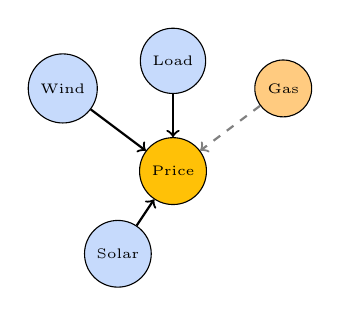
\begin{tikzpicture}[scale=0.7,
    node distance=1cm,
    var/.style={draw, circle, minimum size=0.6cm, font=\tiny}
]
\node[var, fill=elecyellow] (price) at (0,0) {Price};
\node[var, fill=causalblue!30] (wind) at (-2,1.5) {Wind};
\node[var, fill=causalblue!30] (load) at (0,2) {Load};
\node[var, fill=regimeorange!50] (gas) at (2,1.5) {Gas};
\node[var, fill=causalblue!30] (solar) at (-1,-1.5) {Solar};

\draw[->, thick] (wind) -- (price);
\draw[->, thick] (load) -- (price);
\draw[->, thick, dashed, gray] (gas) -- (price);
\draw[->, thick] (solar) -- (price);
\end{tikzpicture}
\end{center}
\textbf{Drivers:} Renewables + Load
\end{column}

\begin{column}{0.5\textwidth}
\textbf{Regime 1 (Crisis/High Volatility):}
\begin{center}
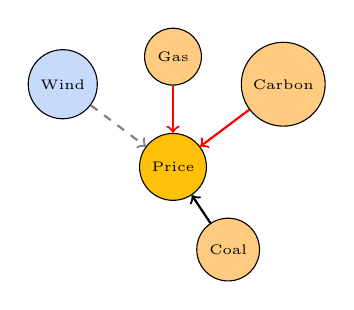
\begin{tikzpicture}[scale=0.7,
    node distance=1cm,
    var/.style={draw, circle, minimum size=0.6cm, font=\tiny}
]
\node[var, fill=elecyellow] (price) at (0,0) {Price};
\node[var, fill=causalblue!30] (wind) at (-2,1.5) {Wind};
\node[var, fill=regimeorange!50] (gas) at (0,2) {Gas};
\node[var, fill=regimeorange!50] (carbon) at (2,1.5) {Carbon};
\node[var, fill=regimeorange!50] (coal) at (1,-1.5) {Coal};

\draw[->, thick, dashed, gray] (wind) -- (price);
\draw[->, thick, red] (gas) -- (price);
\draw[->, thick, red] (carbon) -- (price);
\draw[->, thick] (coal) -- (price);
\end{tikzpicture}
\end{center}
\textbf{Drivers:} Fossil fuels + Carbon
\end{column}
\end{columns}

\vspace{0.2cm}
\begin{center}
\fcolorbox{lightgray}{white}{\parbox{0.9\textwidth}{
\textbf{Legend:} \quad
\tikz{\node[draw, circle, fill=elecyellow, minimum size=0.4cm] {};} Target (Price) \quad
\tikz{\node[draw, circle, fill=causalblue!30, minimum size=0.4cm] {};} Renewable/Load \quad
\tikz{\node[draw, circle, fill=regimeorange!50, minimum size=0.4cm] {};} Commodity (crisis driver)\\[0.1cm]
\quad 
\tikz{\draw[->, thick] (0,0) -- (0.5,0);} Strong causal \quad
\tikz{\draw[->, thick, red] (0,0) -- (0.5,0);} Crisis-dominant \quad
\tikz{\draw[->, thick, dashed, gray] (0,0) -- (0.5,0);} Weak/suppressed
}}
\end{center}
\end{frame}

\begin{frame}{What Drives Price Changes? Regime-Specific DAGs}
\textbf{Interpretation:}
\begin{itemize}
    \item \textbf{Normal regime:} Renewables (wind, solar) and load dominate price formation
    \item \textbf{Crisis regime:} Commodity prices (gas, carbon) become primary drivers
\end{itemize}
\end{frame}

%------------------------------------------------------------------------------
\begin{frame}{Empirical Validation: Detected Regimes Align with Literature}
\begin{columns}
\begin{column}{0.5\textwidth}
\textbf{2021-2022 Energy Crisis (Documented)}
\begin{itemize}
    \item Volatility increased \textbf{159\% in DE}, \textbf{185\% in FR} (2021 vs 2020)
    \item Prices: 35 EUR/MWh (2020) $\rightarrow$ 500+ EUR/MWh (Mar 2022)
    \item ``A clear dividing line between stable pre-crisis and new era of increased volatility'' {\scriptsize [Keles \& Dehler-Holland, 2025]}
\end{itemize}

\vspace{0.2cm}
\textbf{France-Specific Dynamics}
\begin{itemize}
    \item Strongest price increase despite no Russian gas dependence
    \item Nuclear unavailability drove regime change {\scriptsize [Witthaut et al., 2024]}
\end{itemize}
\end{column}

\begin{column}{0.5\textwidth}
\textbf{MRS Models for Electricity (Established)}
\begin{itemize}
    \item Huisman \& Mahieu (2003): First MRS application to DE/UK markets
    \item ``MRS models are a natural candidate for modeling spiky behavior'' {\scriptsize [Janczura \& Weron, 2010]}
    \item Recent: Kapoor \& Balakrishna (2023) use 2-5 regimes for forecasting
\end{itemize}

\vspace{0.2cm}
\textbf{Our Results Align With:}
\begin{itemize}
    \item \textcolor{reprogreen}{\ding{51}} Pre-2021 = Normal regime (low volatility)
    \item \textcolor{reprogreen}{\ding{51}} 2021+ = Crisis regime (high volatility)
    \item \textcolor{reprogreen}{\ding{51}} Gas/commodities as crisis drivers
\end{itemize}
\end{column}
\end{columns}
\end{frame}

%==============================================================================
\begin{frame}{How Does the Setting Matter?}
\begin{columns}
\begin{column}{0.5\textwidth}
\textbf{Task: Estimation vs Prediction}
\begin{itemize}
    \item \textbf{Estimation} ($Y_t | X_{0:t}, Y_{0:t-1}$):
    \begin{itemize}
        \item Higher accuracy (access to recent Y)
        \item Primarily autoregressive signal
        \item Univariate models excel
    \end{itemize}
    \item \textbf{Prediction} ($Y_{t+1} | X_{0:t}, Y_{0:t}$):
    \begin{itemize}
        \item More challenging
        \item CaRS shows \textbf{best directional accuracy} (62-65\%)
        \item Causal structure helps generalize
    \end{itemize}
\end{itemize}
\end{column}

\begin{column}{0.5\textwidth}
\textbf{Target: DE vs FR vs DE\_FR}
\begin{itemize}
    \item \textbf{FR}: Highly autoregressive
    \begin{itemize}
        \item DS3M\_UV achieves $\rho = 0.93$ (d=3)
        \item Nuclear baseload = stable dynamics
    \end{itemize}
    \item \textbf{DE}: More complex
    \begin{itemize}
        \item Higher renewable share
        \item CaRS best for directional prediction
    \end{itemize}
    \item \textbf{DE\_FR}: Joint modeling hardest
    \begin{itemize}
        \item CaRS achieves 55\% directional accuracy
        \item Best among all models
    \end{itemize}
\end{itemize}
\end{column}
\end{columns}

\vspace{0.2cm}
\begin{center}
\fcolorbox{reprogreen}{lightgray}{\parbox{0.9\textwidth}{\centering
\textbf{Recommendations:}\\
\textbf{DS3M\_UV}: Best Spearman for FR (autoregressive)\\
\textbf{CaRS}: Best interpretability for causal analysis\\
\textbf{Shared Backbone}: Best directional accuracy (70-75\%) for trading applications\\
\textbf{Avoid FANTOM\_BEM}: Scalability issues ($>$50 features $\rightarrow$ OOM on 80GB GPU)
}}
\end{center}
\end{frame}

%==============================================================================
\section{Outlook}

\begin{frame}{Future Work}
\begin{columns}
\begin{column}{0.5\textwidth}
\textbf{1. Seed Initialization Variance}
\begin{itemize}
    \item High variance across seeds ($\sigma > 0.1$)
    % \item Is this causal or non-causal?
    \item \textbf{Solutions:}
    \begin{itemize}
        \item Better initialization schemes
        \item Ensemble methods
        \item Bayesian treatment of DAG parameters
    \end{itemize}
\end{itemize}

\vspace{0.3cm}
\textbf{2. Regime Collapse}
\begin{itemize}
    \item Often converges to 1 regime
    \item Need stronger regime regularization
    \item Entropy bonus for regime diversity
\end{itemize}
\end{column}

\begin{column}{0.5\textwidth}
\textbf{3. Additional Data Sources}
\begin{itemize}
    \item \textbf{TTF Gas}: European natural gas benchmark
    \item \textbf{API2 Coal}: Coal price index
    \item \textbf{EU ETS Carbon}: Carbon allowance prices
    \item Weather forecasts, demand forecasts
\end{itemize}

% \vspace{0.3cm}
\textbf{4. Model Enhancements}
\begin{itemize}
    % \item \textbf{Shared Backbone:} Already shows +10-20pp directional accuracy gains
    \item \textbf{Ensembles:} Combine multiple seeds for robust predictions
    \item \textbf{Longer lags:} Currently lag=1, may benefit from lag=2+
\end{itemize}
\end{column}
\end{columns}
\end{frame}

\begin{frame}{Future Work}
\vspace{0.3cm}
\begin{center}
\fcolorbox{causalblue}{lightgray}{\parbox{0.9\textwidth}{\centering
\textbf{Key Challenge:} Balancing model complexity (more regimes, more edges)\\
with stability and interpretability.
}}
\end{center}
\end{frame}

%==============================================================================
\begin{frame}{Summary}
\begin{itemize}
    \item \textbf{CaRS} successfully combines regime switching (DS3M) with causal discovery (FANTOM)

    \item \textbf{Shared Backbone variant} achieves best directional accuracy:
    \begin{itemize}
        \item Prediction: DE \textbf{75\%}, FR \textbf{72-75\%}, DE\_FR \textbf{70-75\%}
        \item Estimation: DE \textbf{78\%}, FR \textbf{76\%}, DE\_FR \textbf{76\%} (d=2)
        \item Consistent across both tasks (small estimation-prediction gap)
    \end{itemize}

    \item \textbf{Key insight:} Shared causal structure improves directional prediction by +8 to +20pp

    \item \textbf{Trade-offs:}
    \begin{itemize}
        \item DS3M\_UV: Best Spearman for autoregressive tasks (FR)
        \item CaRS: Best interpretability with moderate directional accuracy
        \item \textbf{Shared Backbone: Best directional accuracy for trading applications}
    \end{itemize}

    \item \textbf{Open challenges:} Regime collapse, seed variance, Spearman-direction disconnect
\end{itemize}

\vspace{0.3cm}
\begin{center}
\Large\textbf{Questions?}
\end{center}
\end{frame}

%==============================================================================
%==============================================================================
\appendix
\section{Appendix}

%------------------------------------------------------------------------------
\begin{frame}{Appendix: Detailed Literature Review}
\textbf{Regime-Switching Models:}
\begin{itemize}
    \item Hamilton (1989): Markov-switching autoregressive models for business cycles
    \item Kim (1994): Dynamic linear models with regime switching
    \item Xu et al. (2021): \textbf{DS3M} -- Deep Switching State Space Model
\end{itemize}

\vspace{0.2cm}
\textbf{Causal Discovery Methods:}
\begin{itemize}
    \item Spirtes et al. (2000): PC algorithm for constraint-based discovery
    \item Chickering (2002): GES -- Greedy Equivalence Search
    \item Zheng et al. (2018): \textbf{NOTEARS} -- Differentiable DAG learning
    \item Ng et al. (2020): \textbf{GOLEM} -- Likelihood-based structure learning
    \item Pamfil et al. (2020): \textbf{DYNOTEARS} -- Time series extension
\end{itemize}

\vspace{0.2cm}
\textbf{Deep Causal Models:}
\begin{itemize}
    \item Geffner et al. (2022): \textbf{DECI} -- Deep End-to-end Causal Inference
    \item Gong et al. (2022): \textbf{Rhino} -- Historically dependent noise
    \item Rahmani et al. (2025): \textbf{FANTOM} -- Regime-switching causal discovery
\end{itemize}
\end{frame}

%------------------------------------------------------------------------------
\begin{frame}{Appendix: Literature Review (cont.)}
\textbf{Energy Price Modeling:}
\begin{itemize}
    \item Weron (2014): Electricity price forecasting -- comprehensive review
    \item Ziel \& Weron (2018): Day-ahead electricity price forecasting
    \item Lago et al. (2021): Deep learning for electricity price forecasting
    \item Marcjasz et al. (2023): Probabilistic electricity price forecasting
\end{itemize}

\vspace{0.3cm}
\textbf{State Space Models:}
\begin{itemize}
    \item Kalman (1960): Linear state estimation
    \item Durbin \& Koopman (2012): Time series analysis by state space methods
    \item Krishnan et al. (2017): Structured inference networks for nonlinear state space
    \item Rangapuram et al. (2018): Deep state space models for time series forecasting
\end{itemize}

\vspace{0.3cm}
\textbf{Variational Inference:}
\begin{itemize}
    \item Kingma \& Welling (2014): VAE -- Variational Auto-Encoders
    \item Rezende et al. (2014): Stochastic backpropagation
    \item Jang et al. (2017): Gumbel-Softmax for discrete latent variables
\end{itemize}
\end{frame}

%------------------------------------------------------------------------------
\begin{frame}{Appendix: Literature Review (cont.) -- Energy Crisis \& MRS}
\textbf{Energy Crisis \& Regime Validation:}
\begin{itemize}
    \item Keles \& Dehler-Holland (2025): Volatility analysis 2015-2025, MDPI Applied Sciences
    \item Gonzalez-Aparicio et al. (2024): North Sea electricity markets 2018-2022, Energy Economics
    \item Witthaut et al. (2024): Network analysis of 2021-22 crisis, Chaos Journal
    \item Gil-Tertre et al. (2023): Structural changes in energy markets, ECB Forum
\end{itemize}

\vspace{0.3cm}
\textbf{Markov Regime-Switching for Electricity:}
\begin{itemize}
    \item Huisman \& Mahieu (2003): First MRS for electricity prices (DE/UK)
    \item Mount et al. (2006): Predicting price spikes with time-varying MRS, Energy Economics
    \item Janczura \& Weron (2010): Efficient MRS estimation, Computational Statistics
    \item Kapoor \& Balakrishna (2023): MRS forecasting (2-5 regimes), Journal of Forecasting
\end{itemize}

\vspace{0.3cm}
\textbf{Key Finding:} Our detected Normal/Crisis regimes align with documented structural break in European electricity markets starting 2021.
\end{frame}

%------------------------------------------------------------------------------
\begin{frame}{Appendix: Regime Time Series Visualization (DE)}
\begin{center}
\IfFileExists{figures/regime_timeseries_de.svg}{%
    \includesvg[height=0.85\textheight]{figures/regime_timeseries_de.svg}
}{%
    \fcolorbox{lightgray}{white}{\parbox{0.8\textwidth}{\centering
    \vspace{2cm}
    \textbf{[Run generate\_appendix\_plots.py to create figure]}\\[0.5cm]
    Price time series with regime coloring for German market
    \vspace{2cm}
    }}
}
\end{center}
\end{frame}

%------------------------------------------------------------------------------
\begin{frame}{Appendix: Regime Time Series Visualization (FR)}
\begin{center}
\IfFileExists{figures/regime_timeseries_fr.svg}{%
    \includesvg[height=0.85\textheight]{figures/regime_timeseries_fr.svg}
}{%
    \fcolorbox{lightgray}{white}{\parbox{0.8\textwidth}{\centering
    \vspace{2cm}
    \textbf{[Run generate\_appendix\_plots.py to create figure]}\\[0.5cm]
    Price time series with regime coloring for French market
    \vspace{2cm}
    }}
}
\end{center}
\end{frame}

%------------------------------------------------------------------------------
\begin{frame}{Appendix: Regime Time Series Visualization (DE-FR)}
\begin{center}
\IfFileExists{figures/regime_timeseries_de_fr.svg}{%
    \includesvg[height=0.85\textheight]{figures/regime_timeseries_de_fr.svg}
}{%
    \fcolorbox{lightgray}{white}{\parbox{0.8\textwidth}{\centering
    \vspace{2cm}
    \textbf{[Run generate\_appendix\_plots.py to create figure]}\\[0.5cm]
    Price time series with regime coloring for DE-FR spread
    \vspace{2cm}
    }}
}
\end{center}
\end{frame}

%------------------------------------------------------------------------------
\begin{frame}{Appendix: Causal Feature Importance (DE)}
\begin{center}
\IfFileExists{figures/feature_importance_de.svg}{%
    \includesvg[height=0.85\textheight]{figures/feature_importance_de.svg}
}{%
    \fcolorbox{lightgray}{white}{\parbox{0.8\textwidth}{\centering
    \vspace{2cm}
    \textbf{[Run generate\_appendix\_plots.py to create figure]}\\[0.5cm]
    Top causal features for German electricity price
    \vspace{2cm}
    }}
}
\end{center}
\end{frame}

%------------------------------------------------------------------------------
\begin{frame}{Appendix: Causal Feature Importance (FR)}
\begin{center}
\IfFileExists{figures/feature_importance_fr.svg}{%
    \includesvg[height=0.85\textheight]{figures/feature_importance_fr.svg}
}{%
    \fcolorbox{lightgray}{white}{\parbox{0.8\textwidth}{\centering
    \vspace{2cm}
    \textbf{[Run generate\_appendix\_plots.py to create figure]}\\[0.5cm]
    Top causal features for French electricity price
    \vspace{2cm}
    }}
}
\end{center}
\end{frame}

%------------------------------------------------------------------------------
\begin{frame}{Appendix: Causal Feature Importance (DE-FR)}
\begin{center}
\IfFileExists{figures/feature_importance_de_fr.svg}{%
    \includesvg[height=0.85\textheight]{figures/feature_importance_de_fr.svg}
}{%
    \fcolorbox{lightgray}{white}{\parbox{0.8\textwidth}{\centering
    \vspace{2cm}
    \textbf{[Run generate\_appendix\_plots.py to create figure]}\\[0.5cm]
    Top causal features for DE-FR electricity spread
    \vspace{2cm}
    }}
}
\end{center}
\end{frame}

%------------------------------------------------------------------------------
\begin{frame}{Appendix: Lag Analysis}
\begin{center}
\IfFileExists{figures/lag_comparison.svg}{%
    \includesvg[height=0.85\textheight]{figures/lag_comparison.svg}
}{%
    \fcolorbox{lightgray}{white}{\parbox{0.8\textwidth}{\centering
    \vspace{2cm}
    \textbf{[Run generate\_appendix\_plots.py to create figure]}\\[0.5cm]
    Effect of lag on learned graph sparsity\\
    Comparison across lag=1, 2, 3 for DE, FR, DE-FR
    \vspace{2cm}
    }}
}
\end{center}

{\scriptsize \textit{Edge count increases linearly with lag (more temporal connections discovered).}}
\end{frame}

%------------------------------------------------------------------------------
% NEW: Regime-Specific Causal Analysis Results
%------------------------------------------------------------------------------

\begin{frame}{Appendix: Edge Statistics Summary}
\begin{table}
\centering
\scriptsize
\begin{tabular}{l|cc|cc}
\toprule
 & \multicolumn{2}{c|}{\textbf{Germany (DE)}} & \multicolumn{2}{c}{\textbf{France (FR)}} \\
\textbf{Metric} & Regime 0 & Regime 1 & Regime 0 & Regime 1 \\
\midrule
Sample Count & 722 (20\%) & 2929 (80\%) & 697 (19\%) & 2954 (81\%) \\
\midrule
\multicolumn{5}{l}{\textit{Instantaneous Edges (lag=0):}} \\
\quad \# Edges & 420 & 420 & 272 & 272 \\
\quad Avg Weight & 0.000113 & 0.000115 & 0.000124 & 0.000126 \\
\quad Max Weight & 0.000312 & \textbf{0.000462} & 0.000254 & 0.000294 \\
\midrule
\multicolumn{5}{l}{\textit{Lagged Edges (lag=1):}} \\
\quad \# Edges & 441 & 441 & 289 & 289 \\
\quad Avg Weight & 1.21e-06 & 1.25e-06 & 2.22e-06 & 2.22e-06 \\
\quad Max Weight & 3.14e-06 & 5.54e-06 & 4.60e-06 & 4.73e-06 \\
\bottomrule
\end{tabular}
\caption{Edge statistics from DS3MCausal with native Markov regime switching (d=2, lag=1, $\lambda_s$=5.0, seed=42)}
\end{table}

\vspace{0.2cm}
{\scriptsize \textbf{Key observation:} Germany Regime 1 shows significantly higher max instantaneous weight (0.000462), indicating more concentrated causal relationships during crisis periods.}
\end{frame}

%------------------------------------------------------------------------------
\begin{frame}{Appendix: Germany Feature Importance by Regime}
\begin{columns}
\begin{column}{0.48\textwidth}
\textbf{Regime 0 (Normal Market)}
\begin{table}
\scriptsize
\begin{tabular}{l|r}
\toprule
\textbf{Feature} & \textbf{Total Weight} \\
\midrule
Net Flow FR & 0.00498 \\
Fossil Gas & 0.00494 \\
Wind Onshore & 0.00493 \\
Wind 10m & 0.00485 \\
Nat Gas Price & 0.00481 \\
Temperature & 0.00464 \\
Lignite & 0.00463 \\
\bottomrule
\end{tabular}
\end{table}
{\tiny \textit{Renewables + cross-border flows dominant}}
\end{column}

\begin{column}{0.48\textwidth}
\textbf{Regime 1 (Crisis/High Volatility)}
\begin{table}
\scriptsize
\begin{tabular}{l|r}
\toprule
\textbf{Feature} & \textbf{Total Weight} \\
\midrule
\textbf{Actual Load} & \textbf{0.00577} \\
Fossil Gas & 0.00524 \\
Day Ahead Price & 0.00515 \\
Wind 100m & 0.00473 \\
Hydro Pumped & 0.00471 \\
Net Flow FR & 0.00462 \\
Wind Onshore & 0.00460 \\
\bottomrule
\end{tabular}
\end{table}
{\tiny \textit{Load becomes dominant driver (+47\% vs Regime 0)}}
\end{column}
\end{columns}

\vspace{0.3cm}
{\scriptsize Source: \texttt{cars\_de\_d2\_lag1\_ls5.0\_seed42\_ds3m\_causal\_native\_markov.json}}
\end{frame}

%------------------------------------------------------------------------------
\begin{frame}{Appendix: Germany Instantaneous Edges TO Price}
\begin{table}
\centering
\scriptsize
\begin{tabular}{l|c|c|r}
\toprule
\textbf{Feature} & \textbf{Regime 0} & \textbf{Regime 1} & \textbf{Change} \\
\midrule
\textbf{Actual Load} & 0.000107 & \textbf{0.000462} & \textcolor{red}{+332\%} \\
Lignite & 0.0000986 & 0.000174 & \textcolor{red}{+77\%} \\
\midrule
\textbf{Hydro Pumped} & \textbf{0.000140} & 0.000119 & \textcolor{blue}{-15\%} \\
\textbf{Solar} & \textbf{0.000130} & 0.000116 & \textcolor{blue}{-11\%} \\
Nat Gas Price & 0.000129 & 0.000102 & \textcolor{blue}{-21\%} \\
Net Flow FR & 0.000123 & 0.000107 & \textcolor{blue}{-13\%} \\
\midrule
Fossil Gas & 0.000104 & 0.000101 & -3\% \\
Wind Onshore & 0.000104 & 0.0000944 & -9\% \\
Wind Offshore & 0.000103 & 0.000109 & +6\% \\
Nuclear & 0.0000989 & 0.0000994 & +0.5\% \\
\bottomrule
\end{tabular}
\caption{Instantaneous causal edges TO Price (adjacency matrix column 0)}
\end{table}

\vspace{0.2cm}
{\scriptsize \textbf{Interpretation:} During crisis, electricity \textbf{demand (Load)} becomes the overwhelming price driver (4.3$\times$ higher than any other edge), while renewables' influence diminishes.}
\end{frame}

%------------------------------------------------------------------------------
\begin{frame}{Appendix: France Feature Importance by Regime}
\begin{columns}
\begin{column}{0.48\textwidth}
\textbf{Regime 0 (Normal Market)}
\begin{table}
\scriptsize
\begin{tabular}{l|r}
\toprule
\textbf{Feature} & \textbf{Total Weight} \\
\midrule
Wind Offshore & 0.00431 \\
Hydro Pumped & 0.00422 \\
FR Precipitation & 0.00421 \\
Cloud Cover & 0.00419 \\
Nuclear & 0.00416 \\
Wind Onshore & 0.00408 \\
Temperature & 0.00405 \\
\bottomrule
\end{tabular}
\end{table}
{\tiny \textit{Weather + nuclear dominant}}
\end{column}

\begin{column}{0.48\textwidth}
\textbf{Regime 1 (Crisis/High Volatility)}
\begin{table}
\scriptsize
\begin{tabular}{l|r}
\toprule
\textbf{Feature} & \textbf{Total Weight} \\
\midrule
\textbf{Wind 10m} & \textbf{0.00453} \\
FR Radiation & 0.00434 \\
Hydro Pumped & 0.00424 \\
Nuclear & 0.00422 \\
Wind Offshore & 0.00419 \\
Fossil Gas & 0.00415 \\
Actual Load & 0.00412 \\
\bottomrule
\end{tabular}
\end{table}
{\tiny \textit{Weather features increase in importance}}
\end{column}
\end{columns}

\vspace{0.3cm}
{\scriptsize Source: \texttt{cars\_fr\_d2\_lag1\_ls5.0\_seed42\_ds3m\_causal\_native\_markov.json}}
\end{frame}

%------------------------------------------------------------------------------
\begin{frame}{Appendix: France Instantaneous Edges TO Price}
\begin{table}
\centering
\scriptsize
\begin{tabular}{l|c|c|r}
\toprule
\textbf{Feature} & \textbf{Regime 0} & \textbf{Regime 1} & \textbf{Change} \\
\midrule
\textbf{Solar} & 0.000117 & \textbf{0.000161} & \textcolor{red}{+38\%} \\
Nat Gas Price & 0.000116 & 0.000132 & \textcolor{red}{+14\%} \\
Cloud Cover & 0.000107 & 0.000123 & \textcolor{red}{+15\%} \\
\midrule
\textbf{Actual Load} & \textbf{0.000156} & 0.000121 & \textcolor{blue}{-22\%} \\
Wind Offshore & 0.000139 & 0.000110 & \textcolor{blue}{-21\%} \\
Wind 100m & 0.000119 & 0.0000983 & \textcolor{blue}{-17\%} \\
\midrule
Hard Coal & 0.000131 & 0.000119 & -9\% \\
Hydro Pumped & 0.000127 & 0.000123 & -3\% \\
Nuclear & 0.000117 & 0.000111 & -5\% \\
Fossil Gas & 0.000125 & 0.000121 & -3\% \\
\bottomrule
\end{tabular}
\caption{Instantaneous causal edges TO Price (adjacency matrix column 0)}
\end{table}

\vspace{0.2cm}
{\scriptsize \textbf{Interpretation:} France shows a more balanced regime shift -- Solar becomes dominant in crisis regime (+38\%), while Load decreases in importance (-22\%). More subtle structural change than Germany.}
\end{frame}

%------------------------------------------------------------------------------
\begin{frame}{Appendix: Cross-Country Comparison}
\begin{table}
\centering
\scriptsize
\begin{tabular}{l|c|c}
\toprule
\textbf{Metric} & \textbf{Germany (DE)} & \textbf{France (FR)} \\
\midrule
\multicolumn{3}{l}{\textit{Regime Distribution:}} \\
\quad Regime 0 (Normal) & 722 samples (20\%) & 697 samples (19\%) \\
\quad Regime 1 (Crisis) & 2929 samples (80\%) & 2954 samples (81\%) \\
\midrule
\multicolumn{3}{l}{\textit{Regime 0 Top Driver:}} \\
\quad Feature & Hydro Pumped & Actual Load \\
\quad Weight & 0.000140 & 0.000156 \\
\midrule
\multicolumn{3}{l}{\textit{Regime 1 Top Driver:}} \\
\quad Feature & \textbf{Actual Load} & \textbf{Solar} \\
\quad Weight & \textbf{0.000462} & 0.000161 \\
\midrule
\multicolumn{3}{l}{\textit{Regime Differentiation:}} \\
\quad Max weight ratio (R1/R0) & \textbf{4.3$\times$} & 1.0$\times$ \\
\quad Top driver change? & Yes (Hydro $\rightarrow$ Load) & Yes (Load $\rightarrow$ Solar) \\
\bottomrule
\end{tabular}
\end{table}

\vspace{0.3cm}
\textbf{Key Finding:} Germany shows \textbf{dramatic regime differentiation} (Load $\uparrow$ 332\% in crisis), while France shows \textbf{more balanced regimes}. This aligns with Germany's higher gas dependency during the 2021-2022 energy crisis.
\end{frame}

%------------------------------------------------------------------------------
\begin{frame}{Appendix: FANTOM-BEM with Price Returns Target}
\textbf{Motivation:} FANTOM-BEM originally predicts raw Day\_Ahead\_Price (EUR/MWh), while CaRS/DS3M predict price\_change\_pct (returns). We re-ran FANTOM-BEM with returns as the target variable to ensure comparable evaluation.

\vspace{0.3cm}
\begin{table}
\centering
\scriptsize
\begin{tabular}{l|c|c|c|c}
\toprule
\textbf{Market} & \textbf{d=2 Collapse} & \textbf{d=3 Collapse} & \textbf{Edge Count} & \textbf{Top Feature} \\
\midrule
DE & 1/5 (20\%) & 5/5 (100\%) & 127--149 & price\_change\_pct \\
FR & 5/5 (100\%) & 5/5 (100\%) & 82--85 & price\_change\_pct \\
DE\_FR & 5/5 (100\%) & 5/5 (100\%) & 122--124 & price\_spread\_change\_pct \\
\midrule
\textbf{Overall} & \multicolumn{2}{c|}{\textbf{83\% Regime Collapse}} & -- & -- \\
\bottomrule
\end{tabular}
\caption{Regime collapse rates when using price returns as target (5 seeds per config)}
\end{table}

\vspace{0.2cm}
\textbf{Key Finding:} Using returns instead of raw prices causes \textbf{massive regime collapse} (83\% overall). This reveals that the original regime detection was driven by \textbf{price level autocorrelation}, not genuine market regime dynamics.

\vspace{0.2cm}
{\scriptsize \textbf{Implication:} Raw prices exhibit strong autocorrelation that creates spurious temporal structure. Returns remove this autocorrelation, eliminating the signal that differentiated regimes. CaRS avoids this issue by using a different model architecture.}
\end{frame}

%------------------------------------------------------------------------------
\begin{frame}{Appendix: Returns Analysis -- Methodological Insight}
\begin{columns}[T]
\column{0.48\textwidth}
\textbf{Raw Prices (Original)}
\begin{itemize}
    \item Strong autocorrelation ($\rho > 0.9$)
    \item Price levels persist across days
    \item Regime detection captures price ``stickiness''
    \item Distinct regime structure (20/80\% split)
\end{itemize}

\column{0.48\textwidth}
\textbf{Price Returns (New)}
\begin{itemize}
    \item Near-zero autocorrelation
    \item Day-to-day changes are more random
    \item Regime detection loses signal
    \item Regimes collapse to single state
\end{itemize}
\end{columns}

% \vspace{0.4cm}
\begin{table}
\centering
\scriptsize
\begin{tabular}{l|c|c}
\toprule
\textbf{Metric} & \textbf{Raw Prices} & \textbf{Returns} \\
\midrule
Regime Collapse Rate & $<$5\% & 83\% \\
Regime Differentiation & Strong (4.3$\times$) & None \\
RMSE Scale & 12,000--80,000 & $\sim$100--300 \\
Comparable to CaRS? & No & Yes (scale only) \\
\bottomrule
\end{tabular}
\end{table}

% \vspace{0.2cm}
{\scriptsize \textbf{Conclusion:} The regime detection in FANTOM-BEM relies on price level dynamics. When switching to returns, the model cannot identify meaningful regimes, suggesting the Bayesian EM component captures \textit{price persistence patterns} rather than \textit{market state transitions}.}
\end{frame}

%------------------------------------------------------------------------------
\begin{frame}{Appendix: CaRS DAG Learning Ablation Study}
\textbf{Challenge:} The shared backbone architecture produces identical DAGs across regimes.

% \vspace{0.2cm}
\textbf{Ablation experiments} (5 seeds each, mean $\pm$ std):

\begin{table}
\centering
\scriptsize
\begin{tabular}{l|ccc|c}
\toprule
\textbf{Experiment} & \multicolumn{3}{c|}{\textbf{Directional Accuracy (\%)}} & \textbf{DAG L2} \\
 & DE & FR & DE-FR & Diff \\
\midrule
Independent & 74.9$\pm$3.9 & 74.3$\pm$1.5 & 75.1$\pm$1.5 & 0.0 \\
High $\lambda_{diff}$ & \textbf{77.0$\pm$3.9} & \textbf{74.9$\pm$1.3} & \textbf{75.2$\pm$1.0} & 0.0 \\
Noise Init & 74.3$\pm$4.3 & 74.0$\pm$3.7 & 72.9$\pm$4.5 & \textbf{3.6} \\
Combined & 74.4$\pm$4.3 & 74.0$\pm$3.7 & 72.0$\pm$4.2 & \textbf{3.6} \\
\bottomrule
\end{tabular}
\end{table}

% \vspace{0.1cm}
\begin{table}
\centering
\scriptsize
\begin{tabular}{l|ccc|ccc}
\toprule
\textbf{Experiment} & \multicolumn{3}{c|}{\textbf{Regime Balance (R0/R1)}} & \multicolumn{3}{c}{\textbf{Spearman Correlation}} \\
 & DE & FR & DE-FR & DE & FR & DE-FR \\
\midrule
Independent & 266/449 & 406/309 & 429/286 & 0.30 & 0.19 & 0.01 \\
High $\lambda_{diff}$ & 272/443 & 412/303 & 429/286 & \textbf{0.41} & \textbf{0.28} & 0.01 \\
Noise Init & 313/402 & 335/381 & 153/562 & 0.32 & 0.30 & 0.00 \\
Combined & 313/402 & 335/381 & 147/569 & 0.32 & 0.30 & 0.02 \\
\bottomrule
\end{tabular}
\end{table}
\end{frame}

\begin{frame}{Appendix: CaRS DAG Learning Ablation Study}
\textbf{Key Findings:}
\begin{itemize}
    \item \textbf{High $\lambda_{diff}$}: Best accuracy on \textit{all} markets (+2.1\% on DE), most stable
    \item \textbf{Noise init}: Creates DAG differentiation (L2=3.6) but causes regime collapse on DE-FR
    \item \textbf{Trade-off}: DAG differentiation $\leftrightarrow$ accuracy and regime stability
\end{itemize}
\end{frame}

%------------------------------------------------------------------------------
\begin{frame}{Appendix: CaRS DAG Learning -- Edge Statistics}
\textbf{Noise initialization creates regime-specific DAG structures} (seed 42 example):

\vspace{0.3cm}
\begin{columns}[T]
\column{0.48\textwidth}
\textbf{DE Market -- Noise Init}
\begin{table}
\scriptsize
\begin{tabular}{l|cc}
\toprule
\textbf{Metric} & \textbf{Regime 0} & \textbf{Regime 1} \\
\midrule
Mean edge weight & 0.468 & 0.480 \\
Max edge weight & 0.888 & \textbf{0.998} \\
Edges $>$ 0.9 & 0 & \textbf{48} \\
Edges TO Price (max) & 0.864 & \textbf{0.942} \\
\bottomrule
\end{tabular}
\end{table}

\column{0.48\textwidth}
\textbf{FR Market -- Noise Init}
\begin{table}
\scriptsize
\begin{tabular}{l|cc}
\toprule
\textbf{Metric} & \textbf{Regime 0} & \textbf{Regime 1} \\
\midrule
Mean edge weight & 0.601 & 0.615 \\
Max edge weight & 0.901 & \textbf{0.988} \\
Edges $>$ 0.9 & 1 & \textbf{49} \\
Edges TO Price (max) & 0.864 & 0.870 \\
\bottomrule
\end{tabular}
\end{table}
\end{columns}

\vspace{0.4cm}
\textbf{Interpretation:}
\begin{itemize}
    \item Regime 1 develops stronger, more binary edges (closer to 0/1)
    \item DAG L2 difference: 3.6$\pm$0.2 (DE), 3.7$\pm$0.5 (FR) across 5 seeds
    \item \textbf{Trade-off}: DAG differentiation comes at cost of accuracy (--2.7\% on DE)
    \item \textbf{Warning}: Causes regime collapse on DE-FR (153/562 vs 429/286 for high $\lambda$)
\end{itemize}
\end{frame}

%------------------------------------------------------------------------------
\begin{frame}{Appendix: CaRS Architecture Insights}
\textbf{Why does shared backbone fail to differentiate regimes?}

\vspace{0.1cm}
\begin{columns}[T]
\column{0.55\textwidth}
\textbf{Shared Backbone Design:}
\begin{equation*}
A_{\text{regime}_d} = A_{\text{shared}} \oplus A_{\text{deviation}_d}
\end{equation*}
where $\oplus$ is probabilistic OR.

\vspace{0.1cm}
\textbf{Problem:}
\begin{itemize}
    \item Deviations initialized to zero
    \item Gradients from L2 penalty too weak
    \item Both regimes converge to shared backbone
    \item Cosine similarity stays at 1.0
\end{itemize}

\column{0.42\textwidth}
\textbf{Solutions Tested:}
\begin{enumerate}
    \item \textcolor{green}{\ding{51}} Higher $\lambda_{diff}$ (10$\times$)
    \item \textcolor{orange}{\ding{51}} Noise initialization
    \item \textcolor{green}{\ding{51}} Independent DAGs
\end{enumerate}

\vspace{0.1cm}
\textbf{Recommendation:}\\
Use \textbf{high $\lambda_{diff}$} for best directional accuracy across all markets (77.0\% on DE).
\end{columns}

\vspace{0.1cm}
\begin{center}
\fcolorbox{blue!30}{blue!5}{\parbox{0.9\textwidth}{\centering
\textbf{Key Insight:} High $\lambda_{diff}$ achieves best accuracy (77\% on DE) while maintaining regime stability. Noise initialization creates DAG differentiation but degrades performance.
}}
\end{center}
\end{frame}

%------------------------------------------------------------------------------
\begin{frame}{Appendix: Native Markov vs Shared Backbone Configurations}
\begin{columns}[T]
\column{0.48\textwidth}
\textbf{Native Markov / Independent Mode}
\begin{itemize}
    \item \textbf{NOT hierarchical} -- flat structure
    \item $K$ completely independent DAGs
    \item No shared structure across regimes
    \item Each regime: $A_d$ learned independently
\end{itemize}

\vspace{0.2cm}
\begin{center}
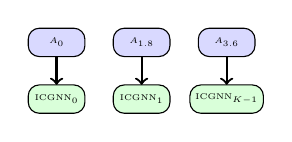
\begin{tikzpicture}[scale=0.6, transform shape]
    \foreach \i/\label in {0/0, 1.8/1, 3.6/K-1} {
        \node[draw, rounded corners, minimum width=1.2cm, minimum height=0.6cm, fill=blue!15] at (\i, 1.2) {\tiny $A_{\i}$};
        \node[draw, rounded corners, minimum width=1.2cm, minimum height=0.6cm, fill=green!15] at (\i, 0) {\tiny ICGNN$_{\label}$};
        \draw[->, thick] (\i, 0.9) -- (\i, 0.3);
    }
\end{tikzpicture}
\end{center}

\column{0.48\textwidth}
\textbf{Shared Backbone Mode}
\begin{itemize}
    \item \textbf{Hierarchical} two-level structure
    \item Global meta DAG: $A_{\text{shared}}$
    \item Regime-specific residuals: $\Delta A_d$
    \item Combined: $A_d = 1 - (1-A_{\text{shared}})(1-\Delta A_d)$
\end{itemize}

\vspace{0.2cm}
\begin{center}
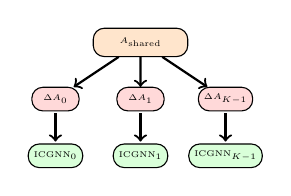
\begin{tikzpicture}[scale=0.6, transform shape]
    \node[draw, rounded corners, minimum width=2cm, minimum height=0.6cm, fill=orange!20] (shared) at (1.8, 2.4) {\tiny $A_{\text{shared}}$};
    \foreach \i/\label in {0/0, 1.8/1, 3.6/K-1} {
        \node[draw, rounded corners, minimum width=1cm, minimum height=0.5cm, fill=red!15] (delta\label) at (\i, 1.2) {\tiny $\Delta A_{\label}$};
        \node[draw, rounded corners, minimum width=1cm, minimum height=0.5cm, fill=green!15] at (\i, 0) {\tiny ICGNN$_{\label}$};
        \draw[->, thick] (\i, 0.9) -- (\i, 0.3);
        \draw[->, thick] (shared) -- (delta\label);
    }
\end{tikzpicture}
\end{center}
\end{columns}

\vspace{0.2cm}
\begin{center}
\fcolorbox{gray!30}{gray!5}{\parbox{0.92\textwidth}{\centering
\textbf{ICGNN:} Both configurations use the \textbf{same CausalICGNN class} with $K$ instances (one per regime).\\
The only difference is the DAG input: composed ($A_{\text{shared}} \oplus \Delta A_d$) vs independent ($A_d$).
}}
\end{center}
\end{frame}

%==============================================================================
%==============================================================================
\section*{Appendix: Mathematical Derivations}
%==============================================================================
%==============================================================================

\begin{frame}{Appendix: ELBO Derivation}
\textbf{Starting Point:} We want to maximize the log-likelihood $\log p(Y|X)$, but it's intractable.

\vspace{0.2cm}
\textbf{Step 1: Introduce variational distribution $q$}
\begin{equation*}
\log p(Y|X) = \log \int p(Y, z, d, G | X) \, dz = \log \int q(z,d,G) \frac{p(Y, z, d, G | X)}{q(z,d,G)} \, dz
\end{equation*}

\textbf{Step 2: Apply Jensen's Inequality} (since $\log$ is concave)
\begin{equation*}
\log p(Y|X) \geq \int q(z,d,G) \log \frac{p(Y, z, d, G | X)}{q(z,d,G)} \, dz = \mathbb{E}_q\left[\log \frac{p(Y, z, d, G | X)}{q(z,d,G)}\right]
\end{equation*}

\textbf{Step 3: Expand the ELBO}
\begin{equation*}
\text{ELBO} = \mathbb{E}_q[\log p(Y|X,z,d,G)] + \mathbb{E}_q[\log p(z,d,G)] - \mathbb{E}_q[\log q(z,d,G)]
\end{equation*}

\textbf{Step 4: Recognize the gap}
\begin{equation*}
\log p(Y|X) = \text{ELBO} + \underbrace{\text{KL}[q(z,d,G) \,\|\, p(z,d,G|Y,X)]}_{\geq 0}
\end{equation*}
\end{frame}

%------------------------------------------------------------------------------
\begin{frame}{Appendix: KL Divergence Computations}
\begin{columns}
\begin{column}{0.5\textwidth}
\textbf{Gaussian KL (closed form):}

For $p = \mathcal{N}(\mu_1, \sigma_1^2)$ and $q = \mathcal{N}(\mu_2, \sigma_2^2)$:
\begin{equation*}
\text{KL}[p \| q] = \log\frac{\sigma_2}{\sigma_1} + \frac{\sigma_1^2 + (\mu_1 - \mu_2)^2}{2\sigma_2^2} - \frac{1}{2}
\end{equation*}

\vspace{0.2cm}
\textbf{For standard normal prior} $q = \mathcal{N}(0, 1)$:
\begin{equation*}
\text{KL}[\mathcal{N}(\mu, \sigma^2) \| \mathcal{N}(0,1)] = -\frac{1}{2}(1 + \log\sigma^2 - \mu^2 - \sigma^2)
\end{equation*}
\end{column}

\begin{column}{0.5\textwidth}
\textbf{Categorical KL:}

For $p = \text{Cat}(\pi)$ and $q = \text{Cat}(\rho)$:
\begin{equation*}
\text{KL}[p \| q] = \sum_{k=1}^{K} \pi_k \log\frac{\pi_k}{\rho_k}
\end{equation*}

\vspace{0.2cm}
\textbf{Application to CaRS:}
\begin{itemize}
    \item $\text{KL}(z_t)$: Uses Gaussian formula with $\mu(h_t, d_t)$, $\sigma(h_t, d_t)$
    \item $\text{KL}(d_t)$: Categorical KL between posterior $q(d_t|h_t,Y_t)$ and Markov prior $p(d_t|d_{t-1})$
\end{itemize}
\end{column}
\end{columns}
\end{frame}

%------------------------------------------------------------------------------
\begin{frame}{Appendix: DAG Acyclicity Constraint (NOTEARS)}
\textbf{Problem:} Ensure learned adjacency matrix $A$ represents a DAG (no directed cycles).

\vspace{0.2cm}
\textbf{Key Insight:} Matrix exponential counts paths of all lengths.
\begin{equation*}
e^A = I + A + \frac{A^2}{2!} + \frac{A^3}{3!} + \ldots
\end{equation*}

\begin{itemize}
    \item $[A^k]_{ij}$ counts paths of length $k$ from $i$ to $j$
    \item Self-loops (cycles): $[A^k]_{ii} > 0$ if node $i$ is on a cycle of length $\leq k$
    \item Trace: $\text{tr}(A^k) = \sum_i [A^k]_{ii}$ sums all self-loops
\end{itemize}

\vspace{0.2cm}
\textbf{NOTEARS Constraint:}
\begin{equation*}
h(A) = \text{tr}(e^{A \odot A}) - n = 0
\end{equation*}

\begin{itemize}
    \item $A \odot A$: Element-wise square (ensures non-negative weights)
    \item If $A$ is a DAG: $\text{tr}(e^{A \odot A}) = n$ (only identity contributes)
    \item If $A$ has cycles: $\text{tr}(e^{A \odot A}) > n$ (cycle terms contribute)
\end{itemize}

\textbf{Optimization:} Augmented Lagrangian: $\mathcal{L} + \lambda h(A) + \frac{\rho}{2}h(A)^2$
\end{frame}

%------------------------------------------------------------------------------
\begin{frame}{Appendix: Gumbel-Softmax Trick}
\textbf{Problem:} Sampling from categorical distribution is not differentiable.

\vspace{0.2cm}
\textbf{Step 1: Gumbel-Max Trick} (exact sampling)
\begin{equation*}
\arg\max_k \left(\log \pi_k + G_k\right) \sim \text{Cat}(\pi), \quad \text{where } G_k \sim \text{Gumbel}(0,1)
\end{equation*}

\textbf{Step 2: Softmax Relaxation} (differentiable approximation)
\begin{equation*}
y_k = \frac{\exp((\log \pi_k + G_k) / \tau)}{\sum_j \exp((\log \pi_j + G_j) / \tau)}
\end{equation*}

\begin{columns}
\begin{column}{0.5\textwidth}
\textbf{Temperature $\tau$ controls sharpness:}
\begin{itemize}
    \item $\tau \to 0$: Approaches hard one-hot samples
    \item $\tau \to \infty$: Approaches uniform distribution
    \item Typical: $\tau = 1.0$ during training
\end{itemize}
\end{column}

\begin{column}{0.5\textwidth}
\textbf{Straight-Through Estimator:}
\begin{itemize}
    \item Forward: Use hard samples (argmax)
    \item Backward: Use soft gradients (softmax)
    \item Enables discrete structure learning
\end{itemize}
\end{column}
\end{columns}

\vspace{0.2cm}
\textbf{In CaRS:} Used for sampling DAG edges $A_{ij} \in \{0,1\}$ in differentiable manner.
\end{frame}

\end{document}
